%\RequirePackage[l2tabu,orthodox]{nag} % This package helps prevent you from doing things wrong.

\documentclass[12pt,a4paper]{article}

\usepackage{ifluatex}
\ifluatex
  \usepackage{fontspec}
  \setmainfont[Ligatures=TeX]{xits}
  %\setmainfont[Ligatures=TeX]{Latin Modern Roman}
  %\fontspec[SmallCapsFeatures={Letters=SmallCaps}]{Latin Modern Roman}
  \setmainfont[
    BoldFont={TeX Gyre Termes Bold},
    ItalicFont={TeX Gyre Termes Italic},
    BoldItalicFont={TeX Gyre Termes Bold Italic},
    Ligatures=TeX,
    SmallCapsFeatures={Letters=SmallCaps}
    ]{TeX Gyre Termes}

% \setmainfont[
%  Ligatures=TeX
%  BoldFont={Minion Pro Bold},
%  ItalicFont={Minion Pro Italic},
%  BoldItalicFont={Minion Pro Bold Italic}
%  ]{Linux Libertine O}

\else
  \usepackage[utf8]{inputenc}
  %\usepackage[T1]{fontenc}
  %\usepackage{times}
\fi

%\usepackage{fontspec}
\usepackage{amsmath, amssymb, mathtools, contmech}
\usepackage{graphicx, subfig, float, grffile}
\usepackage{algorithm, algorithmic}
\usepackage{microtype}
%\usepackage{todonotes}
\usepackage[width=0.8\paperwidth,height=0.85\paperheight]{geometry}
%\usepackage[firstinits=true, style=alphabetic, url=false, isbn=false, hyperref=true]{biblatex}
%\def\bibfont{\footnotesize}
%\usepackage{siunitx}
%\usepackage{fixltx2e}
\usepackage[colorlinks=true,linkcolor=black,citecolor=black]{hyperref}
\usepackage{todonotes}
\usepackage{cleveref}
%\usepackage{showkeys} % Shows equation labels!

\usepackage{tikz, pgfplots}
\usetikzlibrary{arrows}
\pgfplotsset{compat=1.6}
% \renewcommand{\vec}[1]{\mathds{#1}}
% \renewcommand{\mat}[1]{\mathds{#1}}


\ifluatex
  \usepackage{unicode-math}
  %\setmathfont[math-style=ISO]{xits-math.otf}
  %\setmathfont[math-style=ISO]{Asana-Math.otf}
  \setmathfont[math-style=ISO]{latinmodernmath-regular.otf}
  %\setmathfont[math-style=ISO]{texgyretermes-regular.otf}
  \renewcommand{\ta}[1]{\mathbfit{#1}}
  \renewcommand{\ts}[1]{\mathbfit{#1}}
  \renewcommand{\td}[1]{\mathbfcal{#1}}
  \renewcommand{\tf}[1]{\mathbfsfup{#1}}
  \renewcommand{\diff}{\mathbfup{\nabla}}
  \renewcommand{\Box}{\mdlgwhtsquare}
  \renewcommand{\leadsto}{\rightsquigarrow}
\fi

%\captionsetup[subfigure]{textfont=it}
\captionsetup[figure]{textfont=it}
%\newcommand{\figref}[1]{Figure~\ref{#1}}

\linespread{1.3}
\renewcommand{\topfraction}{1.0}	% 99% of page top can be a float
\renewcommand{\bottomfraction}{1.0}	% 99% of page bottom can be a float
\renewcommand{\textfraction}{0.0}	% only 1% of page must to be the text
\renewcommand{\floatpagefraction}{1.0} % 99% of whole page can be a float
\setcounter{totalnumber}{100} %maximum floating objects on one page

% More specialized commands;
\DeclarePairedDelimiter{\homgen}{\langle}{\rangle_\rve}
\DeclarePairedDelimiter{\shomgen}{\langle\!\langle}{\rangle\!\rangle_\rve}
\DeclarePairedDelimiter{\jmp}{[\![}{]\!]}
\newcommand{\prescribed}{\mathrm{pre}}
\newcommand{\on}{\quad\text{ on }}
\renewcommand{\dev}{\mathrm{d}}
\renewcommand{\vol}{\mathrm{v}}
\newcommand{\per}{\mathrm{per}}
\newcommand{\volume}{|\Omega_\rve|}
\newcommand{\ded}{\mathrm{d}}
\newcommand{\dep}{\mathrm{p}}
\newcommand{\Periodic}{\mathrm{P}}

\newcommand{\surf}{\mathrm{s}}
\newcommand{\pore}{\mathrm{pore}}
\newcommand{\particle}{\mathrm{part}}

\newcommand{\epspargs}{\{{\bar{\ts\epsilon}}_\dev, \bar{p}\}}

% Reduce the size of the rve box a bit:
\newcommand{\rve}{
  {\mathchoice
   {\mbox{\scalebox{0.67}{$\Box$}}}
   {\mbox{\scalebox{0.67}{$\Box$}}}
   {\mbox{\scalebox{0.5}{$\Box$}}}
   {\mbox{\scalebox{0.375}{$\Box$}}}
  }
}
\title{Something something porosity}

\author{
Mikael Öhman, Fredrik Larsson and Kenneth Runesson\\
Department of Applied Mechanics \\
Chalmers University of Technology}

\begin{document}
\maketitle
\begin{abstract}
Something
\end{abstract}

\section{Introduction}

Something

The paper is outlined as follows:


\section{Subscale modeling of isotropic elasticity allowing for the incompressible limit}

%\subsection{A mixed $(\ta{u},p)$ weak format}
\subsection{A mixed displacement-pressure weak format}

We consider a generic micro-heterogeneous material in a given body whose macroscopic configuration occupies the region $\Omega$ in space with (presumed smooth) boundary $\Gamma$.
However, the actual medium has porosity, which means the particle composite only occupies only the region $\Omega^\particle$.
We are then lead to defining a Representative Volume Element (RVE), that represents the topology of the micro-heterogeneous microstructure, as shown in \Cref{Figure1}.
The total domain occupied by the cubic RVE is denoted $\Omega_\rve$ with external boundary $\Gamma_\rve$, while particles within the RVE occupies $\Omega_\rve^\particle$.

%-----------------------------------------------------------------------------------------------------------------------------
\begin{figure}
\centering
%\hspace{0.9cm}
%\scalebox{1.0}{
\begin{tikzpicture}
%\tikzstyle{every node}=[font=\Large]
\node [inner sep=0pt,above right]{
   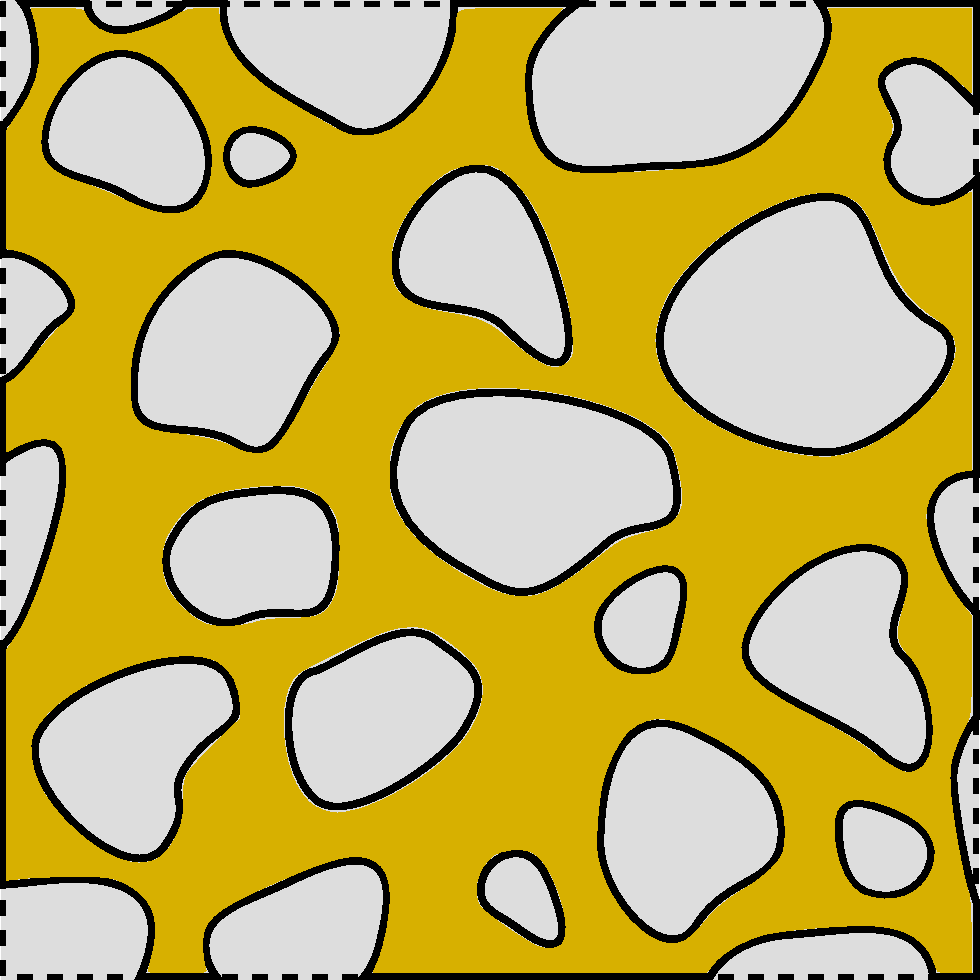
\includegraphics[scale=.3]{SwissCheeseFig}
   };
%\draw[<-, line width=.4mm] (1.6,5.0) .. controls +(up:0.5cm) and +(left:0.5cm) .. (2.5,5.7) node[right=1pt,black,text width=3cm,text badly ragged]{$\Gamma_\rve$};
\draw[<-, line width=.4mm] (5.0,3.5) .. controls +(right:0.5cm) and +(left:0.5cm) .. (6.0,3.5) node[right,black]{$\Gamma_\rve$};
\draw[<-, line width=.4mm] (4.6,2.) .. controls +(right:0.5cm) and +(left:0.5cm) .. (6.0,2.0) node[right,black]{$\Gamma_\rve^\pore$};
%\draw[-*, line width=.4mm] (-1.0,1.5) node[left=-2.0cm,black,text width=3cm,text badly ragged]{$\Omega_{\rve,i}^\mathrm{p}$} .. controls +(right:0.5cm) and +(left:1.cm) .. (0.6,1.1);
\draw[-*, line width=.4mm] (-1.0,2.1) node[left,black]{$\Omega_\rve^\particle$} .. controls +(right:0.5cm) and +(left:1.cm) .. (0.6,2.1);
\draw[-*, line width=.4mm] (-1.0,3.1) node[left,black]{$\Omega_\rve^\pore$} .. controls +(right:0.5cm) and +(left:1.cm) .. (1.2,3.1);
%\draw[<-, line width=.4mm] (4.6,1.7) .. controls +(right:0.5cm) and +(left:0.5cm) .. (6.0,1.0) node[right=1pt,black,text width=3cm,text badly ragged]{$\partial\Omega_{\rve,i}^\text{p}$};
\end{tikzpicture}
%}
\caption{Generic micro-heterogeneous material consisting of inclusions in matrix (example)}
\label{Figure1}
\end{figure}

We consider a model material as follows: The stress is decomposed in terms of deviator and pressure as $\ts{\sigma} = \ts{\sigma}_\dev - p\ts{I}$.
With the kinematic definition $\ts{\epsilon}_\dev[\ta{u}]\defeq[\ta{u}\outerp\diff]^\sym-\frac{1}{3}[\ta{u}\cdot\diff]\ts{I}$, we introduce the constitutive relations
%------------------------------------------------------------------------------------------------------------
\begin{equation}
    \ts{\sigma}_\dev = \hat{\ts{\sigma}}_\dev(\ts{\epsilon}_\dev[\ta{u}]), \quad
    \ta{u}\cdot\diff = \hat{e}(p)
\label{eq201}
\end{equation}
%------------------------------------------------------------------------------------------------------
Hence, $\hat{\ts{\sigma}}_\dev(\bullet)$ and $\hat{e}(\bullet)$ denote suitable constitutive functions.
Obviously, in the simplest case of linear isotropic elasticity, we have $\hat{\ts{\sigma}}_\dev(\ts{\epsilon}_\dev)=2G\ts{\epsilon}_\dev$ and $\hat{e}(p)=-\frac{1}{K}p$, where $G(\ta{x}), K(\ta{x})$ for $\ta{x}\in\Omega$ are the standard elastic moduli that fluctuate strongly.
Moreover, intrinsic incompressibility is defined as $\hat{e}(p)=0$ for any value of $p$.
%------------------------------------------------------------------------------------------------------------------------
We are now in the position to formulate the strong format of the fine-scale problem under standard quasistatic conditions and small strain kinematics:
%------------------------------------------------------------------------------------------------------------
\begin{subequations}\label{eq1}
\begin{alignat}{2}
    -\left[\hat{\ts{\sigma}}_\dev(\ts{\epsilon}_\dev[\ta{u}])-p\ts{I}\right]\cdot\diff & = \ta{f} &&\,\,\text{in}\,\, \Omega^\particle
 \label{eq1a} \\
    -\ta{u}\cdot\diff +  \hat{e}(p) & = 0 &&\,\,\text{in}\,\, \Omega
\label{eq1b} \\
    \ta{t}_\surf \defeq -\kappa\,\gamma_\surf\,\ta n &= \ts\sigma\cdot\ta n &&\,\,\text{on}\,\, \Gamma^\pore
\label{eq1surf} \\
    \ta{u} & = \ta{u}_\prescribed &&\,\,\text{on}\,\, \Gamma^\Dirichlet
\label{eq1c} \\
    \ta{t}\defeq\left[\hat{\ts{\sigma}}_\dev(\ts{\epsilon}_\dev[\ta u])-p\ts{I}\right]\cdot\ta{n} & = \ta t_\prescribed &&\,\,\text{on}\,\, \Gamma^\Neumann
\label{eq1d}
\end{alignat}
\end{subequations}
%-----------------------------------------------------------------------------------------------------
The corresponding weak format is: Find $\ta{u}\in\set{U}, p\in\set{P}$ s.t.
%----------------------------------------------------------------------------------------------------------------
\begin{subequations}\label{eq2}
\begin{alignat}{3}
    a(\ta{u};\delta\ta{u}) + b(p,\delta\ta{u}) &= l_\surf(\delta\ta{u}) + l(\delta\ta{u}) &\quad& \forall \delta\ta{u} &&\in \set{U}^{0}
\label{eq2a} \\
    b(\delta p,\ta{u}) + c^*(p;\delta p) &= 0 &\quad& \forall \delta p &&\in \set{P}
\label{eq2b}
\end{alignat}
\end{subequations}
%----------------------------------------------------------------------------------------------------------------------
where
%----------------------------------------------------------------------------------------------------------------
\begin{align}
    a(\ta{v};\ta{w}) &\defeq
    \int_{\Omega}  \ts{\epsilon}_\dev[\ta{w}]\dprod \hat{\ts{\sigma}}_\dev(\ts{\epsilon}_\dev[\ta{v}]) \dif V
\label{eq3a} \\
    b(q,\ta{v}) &\defeq
    - \int_{\Omega}  q\,\ta{v}\cdot\diff \dif V
\label{eq3b} \\
    c^*(q;r) &\defeq
    \int_{\Omega}  r\,\hat{e}(q) \dif V
\label{eq3c} \\
    l_\surf(\ta{v}) &\defeq -\int_{\Gamma^\pore} \gamma_\surf \hat{\ta I} \dprod [\ta{v}\outerp\diff] \dif S 
\label{eq3d} \\
    l(\ta{v}) &\defeq \int_{\Omega} \ta{v}\cdot\ta{f} \dif V + \int_{\Gamma^\Neumann} \ta{v}\cdot \ta t_\prescribed \dif S
\label{eq3d}
\end{align}
%----------------------------------------------------------------------------------------------------------------------
The solution space $\set{U}$ and the test space $\set{U}^0$ are defined in standard fashion.
In particular, all $\ta{v}\in\set{U}$ are characterized by $\ta{v}=\ta{u}_\prescribed$ on $\Gamma^\Dirichlet$, whereas all $\ta{v}\in\set{U}^0$ satisfy $\ta{v}=\ta{0}$ on $\Gamma^\Dirichlet$.
The pressure space $\set{P}$ does not satisfy any boundary conditions.

It is illuminating (although not necessary from an operational point of view) to invoke the potential $\Pi(\ta{u},p)$
%----------------------------------------------------------------------------
\begin{align}
    \Pi(\ta{u},p) &\defeq \Lambda(\ta{u},p) - l_\surf(\ta{u}) - l(\ta{u})
    \quad\mbox{with}\quad
    \Lambda(\ta{u},p) \defeq \int_{\Omega} \left[\psi_\mathrm{u}(\ts{\epsilon}_\dev[\ta{u}]) - p\,\ta{u}\cdot\diff + \psi_\mathrm{p}^*(p)\right] \dif V
\label{eq121}
\end{align}
%----------------------------------------------------------------------------
where $\psi_u(\ts{\epsilon}_\dev)$ and $\psi_p^*(p)$ are constitutive energy densities\footnote{* indicates ``complementary energy''} such that
%----------------------------------------------------------------------------
\begin{align}
    \hat{\ts{\sigma}}_\dev(\ts{\epsilon}_\dev)=\frac{\partial\psi_\mathrm{u}(\ts{\epsilon}_\dev)}{\partial\ts{\epsilon}_\dev}, &\quad
    \hat{e}(p)=\frac{\partial\psi_\mathrm{p}^*(p)}{\partial p}
\label{eq122}
\end{align}
%----------------------------------------------------------------------------
The stationarity conditions of $\Pi(\ta{u},p)$ are
%----------------------------------------------------------------------------------------------------------------
\begin{subequations}\label{eq123}
\begin{alignat}{3}
    \Pi'_u(\ta{u},p;\delta\ta{u}) &= a(\ta{u};\delta\ta{u}) + b(p,\delta\ta{u})- l_\surf(\delta\ta{u})  - l(\delta\ta{u}) =0 &\quad& \forall \delta\ta{u} &&\in \set{U}^{0}
\label{eq123a} \\
    \Pi'_p(\ta{u},p;\delta p) &= b(\delta p,\ta{u}) + c^*(p;\delta p) = 0 &\quad& \forall \delta p &&\in \set{P}
\label{eq123b}
\end{alignat}
\end{subequations}
%----------------------------------------------------------------------------------------------------------------------
which are identical to the weak form in \cref{eq2}.

\section{Variationally Consistent Homogenization}

\subsection{VMS-ansatz and scale separation}

The appropriate variational setting of the homogenized problem is obtained upon replacing the integrands in the weak forms in \crefrange{eq3a}{eq3d} by running averages of the type
%----------------------------------------------------------------------------
\begin{align}
    y \mapsto
    \homgen{y} &\defeq \frac{1}{\volume}\int_{\Omega_\rve^\particle} y \dif V, \quad \Omega_\rve^\particle = \Omega^\particle \cap\Omega_\rve
    \label{eq16ba}
\intertext{and for the internal surface $\Gamma^\pore$}
    y \mapsto
    \shomgen{ y } &\defeq \frac{1}{\volume}\int_{\Gamma_\rve^\pore} y \dif S, \quad \Gamma_\rve^\pore = \Gamma^\pore \cap\Omega_\rve
    \label{eq16ba}
\end{align}
%----------------------------------------------------------------------------
representing a smoothing approximation on a RVE.
In practice, the RVE's are finite-sized and occupies the subscale region $\Omega_\rve$ with boundary $\Gamma_\rve$.
The typical dimension of an RVE is $L_\rve=\volume^{1/3}$.
The RVE is centered at the macroscale position $\bar{\ta{x}}\defeq\frac{1}{|\Gamma_\rve|}\int_{\Gamma_\rve} \ta{x}\dif S$ for any given $\bar{\ta{x}}\in\Omega$.
Boundary integrals can be homogenized in similar fashion, by considering Representative Surface Elements $\Gamma_\#$
\begin{align}
 y \to \langle y \rangle_{\#} \defeq \frac{1}{|\Gamma_\#|} \int_{\Gamma_\#} y \dif S
\end{align}


The weak forms in \crefrange{eq3a}{eq3d} are thus approximated as
%----------------------------------------------------------------------------------------------------------------
\begin{align}
    a(\ta{v};\ta{w}) &\approx \int_\Omega a_\rve(\ta{v};\ta{w}) \dif V
\label{eq7a} \\
    b(q,\ta{v}) &\approx \int_\Omega b_\rve(q,\ta{v}) \dif V
\label{eq7b} \\
    c^*(q;r) &\approx \int_\Omega c^*_\rve(q;r) \dif V
\label{eq7c} \\
    l(\ta{v}) &\approx \int_\Omega l_\rve(\ta{v}) \dif V + \int_{\Gamma^\Neumann} l_\#(\ta{v}) \dif S
\label{eq7d} \\
    l_\surf(\ta{v}) &\approx \int_\Omega l_{\surf\rve}(\ta v) \dif V
\label{eq7e}
\end{align}
%---------------------------------------------------------------------------------------------------------------------
where the RVE-functionals in \crefrange{eq7a}{eq7d} are defined as
%----------------------------------------------------------------------------------------------------------------
\begin{align}
    a_\rve(\ta{v};\ta{w}) &\defeq
    \homgen{ \ts{\epsilon}_\dev[\ta{w}]\dprod \hat{\ts{\sigma}}_\dev(\ts{\epsilon}_\dev[\ta{v}]) }
\label{eq8a} \\
    b_\rve(q,\ta{v}) &\defeq
    -  \homgen{ q\,\ta{v}\cdot\diff }
\label{eq8b} \\
    c^*_\rve(q;r) &\defeq
    \homgen{ r\,\hat{e}(q) }
\label{eq8c} \\
    l_{\surf\rve}(\ta{v}) &\defeq
    \shomgen{ \gamma_\surf \hat{\ts I} \dprod [\ta{v}\outerp\diff] }
\label{eq8d} \\
    l_\rve(\ta{v}) &\defeq
    \homgen{ \ta{v}\cdot\ta{f} }, \quad
    l_\#(\ta{v}) \defeq
    \langle \ta{v}\cdot \ta t_\prescribed \rangle_\#
\label{eq8e}
\end{align}
%---------------------------------------------------------------------------------------------------------------------
Likewise, we homogenize the volume-specific energy potential $\Lambda(\ta{u},p)$:
%----------------------------------------------------------------------------
\begin{align}
    \Lambda(\ta{v},q) &\approx \int_\Omega \Lambda_\rve(\ta{v},q) \dif V
\label{eq222}
\end{align}
%----------------------------------------------------------------------------
where the RVE-functional $\Lambda_\rve(\ta{v},q)$ is given as
%----------------------------------------------------------------------------
\begin{align}
    \Lambda_\rve(\ta{v},q) &\defeq
    \homgen{ \psi_u(\ts{\epsilon}_\dev[\ta{v}])}
    + l_{\surf\rve}(\ta{v}) 
    - \homgen{  p\,\ta{v}\cdot\diff } + \homgen{ \psi_p^*(q) }
\label{eqRveBulkPotential}
\end{align}
%----------------------------------------------------------------------------
Note in particular the treatment of the surface tension in \cref{eq7e}, which exists now only in the RVE-problem, and influences the macroscale problem only through \cref{eq7a, eq7b}.

In the spirit of the Variational MultiScale method (VMS) \cite{larsson_variationally_2010}, we introduce the \emph{ansatz} that the fields $\ta{u}\in\set{U}$ and $p\in\set{P}$ can be decomposed into macroscale (smooth) and subscale (fluctuating) parts inside each RVE via the unique orthogonal split $\set{U} = \set{U}^\macro \oplus \set{U}^\fluct$ and $\set{P} = \set{P}^\macro \oplus \set{P}^\fluct$.
As a result, we may assume that it is possible solve for the fluctuation fields $\ta{u}^\fluct\in\set{U}^\fluct$ and $p^\fluct\in\set{P}^\fluct$ as ``local approximations'' on each RVE for given macroscale solutions $\ta{u}^\macro\in\set{U}^\macro$ and $p^\macro\in\set{P}^\macro$, i.e.\ we construct the complete solution on each RVE as\footnote{Curly brackets $\{(\bullet)\}$ indicate implicit and/or nonlocal functional dependence on $(\bullet)$.}.
%------------------------------------------------------------------------------------------------------------
\begin{subequations}\label{eq4}
\begin{alignat}{2}
    \ta{u}\approx \tilde{\ta{u}}\{\ta{u}^\macro,p^\macro\} &\defeq \ta{u}^\macro+\tilde{\ta{u}}^\fluct\{\ta{u}^\macro,p^\macro\} &&\text{ in } \Omega_\rve
\label{eq4a} \\
    p\approx \tilde{p}\{\ta{u}^\macro,p^\macro\} &\defeq p^\macro+\tilde{p}^\fluct\{\ta{u}^\macro,p^\macro\} &&\text{ in } \Omega_\rve
\label{eq4b}
\end{alignat}
\end{subequations}
%------------------------------------------------------------------------------------------------------------
On the boundary of the macroscale domain, $\Gamma$, we assume smooth variation of $\ta{u}$ defined by the explicit relations $\ta u = \ta u^\macro$, $p = p^\macro$ on $\Gamma_\#$.


In addition, the test function $\delta\ta{u}\in\set{U}^{0}$ in \cref{eq2a} is replaced by $\delta\ta{u}^\macro\in\set{U}^{\macro,0}$, whereas $\delta p\in\set{P}$ in \cref{eq2b} is replaced by $\delta p^\macro\in\set{P}^{\macro}$.
Altogether, these assumptions infer that $\ta{u}^\macro\in\set{U}^\macro$ and $p^\macro\in\set{P}^\macro$ can be solved from the homogenized problem
%----------------------------------------------------------------------------------------------------------------
\begin{subequations}\label{eq6}
\begin{alignat}{3}
    a(\tilde{\ta{u}}\{\ta{u}^\macro,p^\macro\};\delta\ta{u}^\macro) +
    b(\tilde{p}\{\ta{u}^\macro,p^\macro\},\delta\ta{u}^\macro)
    &= l(\delta\ta{u}^\macro)
    &\quad& \forall \delta\ta{u}^\macro &&\in \set{U}^{\macro,0}
\label{eq6a} \\
    b(\delta p^\macro,\tilde{\ta{u}}\{\ta{u}^\macro,p^\macro\}) +
    c^*(\tilde{p}\{\ta{u}^\macro,p^\macro\};\delta p^\macro)
    &= 0 &\quad& \forall \delta p^\macro &&\in \set{P}^{\macro}
\label{eq6b}
\end{alignat}
\end{subequations}
%----------------------------------------------------------------------------------------------------------------------

\subsection{Explicit format of macroscale (homogenized) problem}
In practice, the scales are linked  by expressing $\ta{u}^\macro(\bar{\ta{x}},{\ta{x}})$\footnote{Double arguments, i.e.\ $\ta{u}(\bar{\ta{x}},\ta{x})$, are used to explicitly point out the underlying scale separation.} and $p^\macro(\bar{\ta x},\ta x)$ using Taylor series expansions of suitable order for $\bar{\ta{x}}\in\Omega$ and $\ta{x}\in\Omega_\rve(\bar{\ta{x}})$
in terms of the macroscale solution $\bar{\ta{u}}(\bar{\ta{x}})$ and $\bar{p}(\bar{\ta x})$ respectively.
We thus introduce the macroscale fields $(\bar{\ta{u}},\bar{p})\in\bar{\set{U}}\times\bar{\set{P}}$ such that the macroscale solutions $\ta{u}^\macro, p^\macro$ inside each RVE are expanded as follows:
%----------------------------------------------------------------------------
\begin{subequations}\label{eq12}
\begin{align}
    \ta{u}^\macro(\bar{\ta{x}};\ta{x}) &= \bar{\ta{u}}(\bar{\ta{x}}) + \bar{\ts{h}}(\bar{\ta{x}}) \cdot [\ta{x}-\bar{\ta{x}}], \quad \bar{\ts{h}}\defeq\bar{\ta{u}}\outerp\diff, \quad \ta{x}\in\Omega_\rve
\label{eq12a} \\
    p^\macro(\bar{\ta{x}};\ta{x}) &= \frac{|\Omega_\rve|}{|\Omega_\rve^\particle|} [\bar{p}(\bar{\ta{x}}) + \frac23 \shomgen{\gamma_\surf}] \quad
    \ta{x}\in\Omega_\rve
\label{eq12b}
\end{align}
\end{subequations}
%----------------------------------------------------------------------------
Hence, $\ta{u}^\macro$ is assumed to have linear variation in $\Omega_\rve$ pertinent to standard ``first order homogenization'', whereas $p^\macro$ is constant in $\Omega_\rve$.
Now, we require that
%----------------------------------------------------------------------------
\begin{subequations}\label{eq14}
\begin{gather}
    \frac{1}{|\Gamma_\rve|} \int_{\Gamma_\rve} \ta{u} \dif S = \bar{\ta{u}}, \quad
    \frac{1}{\volume} \int_{\Gamma_\rve} \ta{u} \outerp \ta n \dif V = \bar{\ta{h}}
\label{eq14a} \\
    %\frac{1}{\volume} \int_{\Gamma_\rve} p\,\ta n \cdot [\ta x-\bar{\ta x}] \dif S = \bar{p}
    \homgen{p} - \frac23 \shomgen{\gamma_\surf} = \bar{p}
\label{eq14b}
\end{gather}
\end{subequations}
which leads to the constraints
%----------------------------------------------------------------------------
\begin{subequations}\label{eq13}
\begin{gather}
    \frac{1}{|\Gamma_\rve|} \int_{\Gamma_\rve} \ta{u}^\fluct \dif S = \ta 0, \quad
    \frac{1}{\volume} \int_{\Gamma_\rve} \ta{u}^\fluct \outerp \ta n \dif V = \ts 0
\label{eq14a} \\
    \homgen{p^\fluct} = 0
\label{eq14b}
\end{gather}
\end{subequations}
%----------------------------------------------------------------------------
As a result, the hierarchical split ($\set{U} = \set{U}^\macro \oplus \set{U}^\fluct$ and $\set{P} = \set{P}^\macro \oplus \set{P}^\fluct$) is guaranteed.
%----------------------------------------------------------------------------
We can thus establish at the outset, before any further analysis, that the displacement and pressure fields within each RVE are implicit functions of the values $\bar{\ta u}$, $\bar{\ts h}$, $\bar{p}$, such that $\ta u = \tilde{\ta u}\{\bar{\ta u}, \bar{\ts h}, \bar{p}\}$ and $p = \tilde{p}\{\bar{\ta u}, \bar{\ts h}, \bar{p}\}$.

With the representations in \cref{eq12} and the constraints in \cref{eq14,eq13}, we are in the position to compute the homogenized quantities that enter the system \cref{eq6}:
%----------------------------------------------------------------------------------------------------------------
%\todo{$\delta u^\macro$ in RHS but not in LHS}
\begin{align}
    a_\rve(\ta{u};\delta\ta{u}^\macro) &=
    \homgen{ \hat{\ts{\sigma}}_\dev(\ts{\epsilon}_\dev[\ta{u}]) } \dprod \ts{\epsilon}_\dev[\delta\bar{\ta{u}}] 
\label{eq15a} \\
    b_\rve(p,\delta\ta{u}^\macro) &=
    -  \homgen{ p }\, \delta\bar{\ta{u}}\cdot\diff
\label{eq15b} \\
    b_\rve(\delta p^\macro,\ta{u}) &=
    - \frac{|\Omega_\rve|}{|\Omega_\rve^\particle|}\delta\bar{p}\, \homgen{ \ta{u}\cdot\diff } = - \delta\bar{p} \, \bar{\ta u}\cdot\diff - \frac{|\Omega_\rve|}{|\Omega_\rve^\particle|}\delta\bar{p}\,\homgen{ \ta{u}^\fluct\cdot\diff }
\label{eq15c} \\
    c^*_\rve(p;\delta p^\macro) &=
    \frac{|\Omega_\rve|}{|\Omega_\rve^\particle|}\delta\bar{p}\, \homgen{ \hat{e}(p) }
\label{eq15d} \\
    l_{\surf\rve}(\delta\ta{u}^\macro) &=
    -\shomgen{ \gamma_\surf \hat{\ts I} } \dprod [\delta\bar{\ta{u}}\outerp\diff]
\label{eq15e} \\
    l_\rve(\delta\ta{u}^\macro) &=
    \delta\bar{\ta{u}}\cdot \bar{\ta f} + [\delta\bar{\ta{u}}\outerp\diff]\dprod \bar{\bar{\ta f}}
\label{eq15f} \\
    l_\#(\delta\ta{u}^\macro) &=
    \delta\bar{\ta{u}} \cdot \bar{\ta t}_\prescribed + [\delta\bar{\ta u}\outerp\diff]\dprod \bar{\bar{\ta{t}}}_\prescribed
\label{eq15g}
\end{align}
%---------------------------------------------------------------------------------------------------------------------
The applied macroscale loads $\bar{\ta f}$, $\bar{\ta t}_\prescribed$ and ``moments'' $\bar{\bar{\ta f}}$, $\bar{\bar{\ta t}}_\prescribed$ are defined as
%----------------------------------------------------------------------------------------------------------------
\begin{alignat}{2}
    \bar{\ta f} &= \homgen{ \ta{f} },\quad
    &\bar{\bar{\ta f}} &= \homgen{ \ta{f}\outerp[\ta{x}-\bar{\ta{x}}] }
\label{eq15fa}
\\
    \bar{\ta t}_\prescribed &= \langle \ta{t}_\prescribed \rangle_\#,\quad
    &\bar{\bar{\ta t}}_\prescribed &= \langle \ta{t}_\prescribed\outerp[\ta{x}-\bar{\ta{x}}]  \rangle_\#
\end{alignat}
%---------------------------------------------------------------------------------------------------------------------
\textbf{Remark:} Henceforth, we restrict to the situation when $\volume\to 0$ and $|\Gamma_\#|\to 0$; hence $\bar{\bar{\ta f}}$ and $\bar{\bar{\ta t}}_\prescribed$ will vanish.
We will also focus on the homogenization of $\bar{\ts\sigma}_\dev$ and $\bar{e}$, so $\bar{\ta f}$ and $\bar{\ta t}_\prescribed$ are considered as given macroscopic quantities. $\Box$

Plugging \cref{eq15a,eq15b,eq15c,eq15d,eq15e,eq15f,eq15g} into \cref{eq6} weak form we get
\begin{subequations}\label{eq:derived_macro}
\begin{align}
 \int_\Omega \underbrace{[\homgen{ \hat{\ts{\sigma}}_\dev(\ts{\epsilon}_\dev[\ta{u}]) - p \ts I } + \shomgen{ \gamma_\surf \hat{\ts I}}]}_{=\bar{\ts\sigma}_\dev - \bar{p}\ts I} \dprod [\delta\bar{\ta{u}}\outerp\diff] \dif V &= 
  \int_\Omega \bar{\ta f} \cdot \delta\bar{\ta u} \dif V + 
  \int_\Gamma \bar{\ta t}_\prescribed \cdot \delta\bar{\ta u} \dif S
\label{eq:derived_macro_a}
\\
 \int_\Omega \Big[ - \delta\bar{p}\, \bar{\ta{u}}\cdot\diff + \delta\bar{p}\, \underbrace{\frac{|\Omega_\rve|}{|\Omega_\rve^\particle|}\homgen{ \hat{e}(p) - \ta u^\fluct\cdot\ta n}}_{\bar{e}} \Big]\dif V &= 0
\label{eq:derived_macro_b}
\end{align}
\end{subequations}
where we continue to manipulate \cref{eq:derived_macro_a} further
\begin{align}
 \homgen{ \hat{\ts{\sigma}}_\dev(\ts{\epsilon}_\dev[\ta{u}]) - p \ts I } + \shomgen{ \gamma_\surf \hat{\ts I}}
  = \homgen{ \ts{\sigma} } + \shomgen{ \gamma_\surf \hat{\ts I}}
\nonumber\\
  = \frac{1}{\volume} \Big[ \int_{\Gamma_\rve \cup \Gamma_\rve^\pore } \ta t \outerp[\ta x-\bar{\ta x}] \dif S + \shomgen{ \gamma_\surf \hat{\ts I}} \Big]
\nonumber\\
  = \frac{1}{\volume} \Big[\int_{\Gamma_\rve} \ta t \outerp[\ta x-\bar{\ta x}] \dif S + \int_{\Gamma_\rve^\pore } [\ta t_\surf \outerp[\ta x-\bar{\ta x}] + \gamma_\surf \hat{\ts I} ]\dif S \Big]
\nonumber\\
  = \frac{1}{\volume} \Big[\int_{\Gamma_\rve} \ta t \outerp[\ta x-\bar{\ta x}] \dif S + \int_{\partial\Gamma_\rve^\pore} \hat{\ta t}\outerp[\ta x - \bar{\ta x}]\dif C \Big]
 \label{eq:derived_macro_a2}
\end{align}
Since pore boundaries on $\Gamma_\rve$ is not applicable for the weakly periodic or Neumann boundary condition, we henceforth limit the RVE's to have no pores crossing the boundary $\Gamma_\rve$, and as such the integral over $\partial\Gamma_\rve^\pore$ also vanishes. Thus we are in position to define the macroscopic deviatoric stress and volumetric strain
%----------------------------------------------------------------------------------------------------------------
\begin{align}
    \bar{\ts{\sigma}}_\dev \defeq \frac{1}{\volume}\int_{\Gamma_\rve} \ta t \outerp[\ta x-\bar{\ta x}] \dif S + \bar{p}\ts I, \, \quad
    \bar{e} \defeq \frac{|\Omega_\rve|}{|\Omega_\rve^\particle|}\homgen{ \hat{e}(p) - \ta u^\fluct\cdot\diff}
\label{eq16}
\end{align}
%----------------------------------------------------------------------------------------------------------------
We note that $\bar{\ts\sigma}_\dev$ and $\bar{e}$ are indeed implicit functions of the values of the macroscale variables $\bar{\ta u}$, $\bar{\ts h}$ and $\bar{p}$, pertinent to the considered RVE.

\noindent\textbf{Remark:} If one wants to include a non-empty $\partial\Gamma_\rve^\pore$, then \cref{eq14b} also needs to include the corresponding term in order obtain the same macroscopic problem. $\Box$

Finally, we may express the macroscale problem the abstract form:
Find $(\bar{\ta{u}},\bar{p})\in\bar{\set{U}}\times\bar{\set{P}}$ that solve
%----------------------------------------------------------------------------------------------------------------
\begin{subequations}\label{eq:derived_macro}
\begin{alignat}{3}
    \bar{a}(\bar{\ta{u}},\bar{p};\delta\bar{\ta{u}}) + \bar{b}(\bar{p},\delta\bar{\ta{u}}) &= \bar{l}(\delta\bar{\ta{u}})
      &\quad& \forall \delta\bar{\ta{u}} &&\in \bar{\set{U}}^{0}
\label{eq:derived_macro_a} \\
    \bar{b}(\delta\bar{p},\bar{\ta{u}}) + \bar{c}^*(\bar{\ta{u}},\bar{p};\delta\bar{p}) &= 0
      &\quad& \forall \delta\bar{p} &&\in \bar{\set{P}}
\label{eq:derived_macro_b}
\end{alignat}
\end{subequations}
%----------------------------------------------------------------------------------------------------------------------
where
%----------------------------------------------------------------------------------------------------------------
\begin{align}
    \bar{a}(\bar{\ta{u}},\bar{p};\bar{\ta w}) &\defeq
    \int_{\Omega}  \ts{\epsilon}_\dev[\bar{\ta w}]\dprod\bar{\ts\sigma}_\dev\{\bar{\ta u}, \bar{p}\} \dif V
\label{eq18a} \\
    \bar{b}(\bar{q},\bar{\ta u}) &\defeq
    - \int_{\Omega}  \bar{q}\,\bar{\ta{u}}\cdot\diff \dif V
\label{eq18b} \\
    \bar{c}^*(\bar{\ta{u}},\bar{p};\bar{r}) &\defeq
    \int_{\Omega}  \bar{r}\,\bar{e}\{\bar{\ta u}, \bar{p}\} \dif V
\label{eq18c} \\
    \bar{l}(\bar{\ta u}) &\defeq  \int_{\Omega}  \bar{\ta u}\cdot\bar{\ta f} \dif V +
    \int_{\Gamma^\Neumann} \bar{\ta u}\cdot\bar{\ta t}_\prescribed \dif S
\label{eq18d}
\end{align}
%----------------------------------------------------------------------------------------------------------------------
If we consider the macroscale fields, $\bar{\ts\sigma}_\dev$ and $\bar{e}$,  we conclude that they are implicit functions of the fields $\bar{\ta u}$ and $\bar{p}$.
The macroscale spaces $\bar{\set{U}}$ and $\bar{\set{P}}$ are chosen as the standard ones for the fine-scale problem.

\section{Canonical formulation of RVE-problem}

\subsection{Preliminaries -- Concept of weak periodicity of fluctuation displacement}

To avoid unnecessary technical complexity, we henceforth consider the situation without volume load, i.e.\ $\ta{f}=\ta{0}$.
As a preliminary for establishing the proper variational format of the RVE-problem, we consider the most general weak form of the quasi-static momentum balance by introducing the boundary integral with boundary tractions:
%----------------------------------------------------------------------------
\begin{subequations}
\begin{align}
    a_\rve(\ta{u};\delta\ta{u}) + b_\rve(\delta\ta{u},p) - \frac{1}{\volume}\int_{\Gamma_\rve} \ta{t}\cdot\delta\ta{u} \dif S &= l_{\fluct\rve}(\delta\ta{u})
\label{eq19a} \\
    b_\rve(\ta{u},\delta p) + c^*_\rve(p;\delta p) &= 0
\label{eq19b}
\end{align}
\end{subequations}
%---------------------------------------------------------------------------
which is supposed to hold true for all possible $\delta\ta{u}, \delta p$ in suitable function spaces (as discussed below).
However, this problem is not solvable without further specification of the solution fields $\ta{u}, p, \ta{t}$.
In this paper we adopt a recently proposed variational framework allowing for \emph{weak satisfaction of micro-periodicity}, cf.\  Larsson et al.\ \cite{larsson_computational_2011}, and this framework will be briefly summarized in what follows.
We then \emph{assume} that the subscale fluctuation field $\ta{u}^\fluct$ is periodic across the RVE boundaries w.r.t.\ the chosen local coordinate axes.
This model assumption, which may be termed ``micro-periodicity'', is a key ingredient (and frequently adopted) in the literature on mathematical homogenization and can be viewed as an approximation between the stiffer Dirichlet and the weaker Neumann boundary conditions.
Indeed, both these cases can be obtained as special cases of the most general variational format of periodicity (as will be discussed further below).

In order to formulate the conditions on micro-periodicity, we consider the RVE in \cref{Figure2}, where the boundary $\Gamma_\rve$ has been split into two parts: $\Gamma_\rve=\Gamma_\rve^- \cup \Gamma_\rve^+$.
Here, $\Gamma_\rve^+$ is the \emph{image boundary} (later chosen as the computational domain for boundary integration), whereas $\Gamma^-$ is the \emph{mirror boundary}.
We shall now introduce the proper mapping $\ta{\varphi}_\per:\Gamma^+ \rightarrow \Gamma^-$ such that any point $\ta{x}^+\in\Gamma_\rve^+$ is mirrored in a self-similar fashion to the corresponding point $\ta{x}^-\in\Gamma_\rve^-$; hence, $\ta{x}^-=\ta{\varphi}_\per(\ta{x}^+)$.
%---------------------------------------------------------------------------------
\begin{figure}[H]
\centering
\begin{tikzpicture}
%\tikzstyle{every node}=[font=\Large]
\node [inner sep=0pt,above right]{
   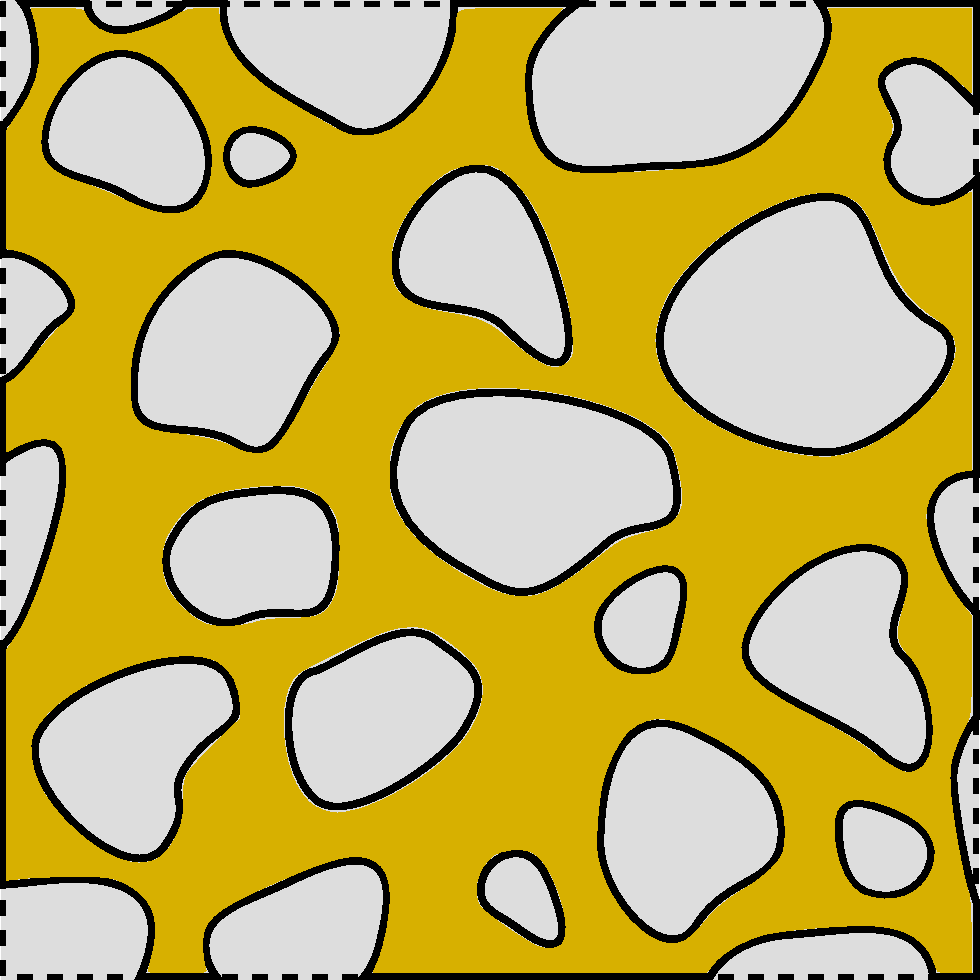
\includegraphics[scale=.3]{SwissCheeseFig}
   };
\draw[<-, line width=.4mm] (5.0,4.0) to[out=0,in=-120] (6.0,5.0) node[right=1pt,black]{$\Gamma_\rve^+$};
\draw[<-, line width=.4mm] (4.0,5.0) to[out=60,in=120] (6.0,5.0);
\draw[<-, line width=.4mm] (0.0,1.0) to[out=180,in=60] (-1.0,0.0) node[left=1pt,black]{$\Gamma_\rve^-$};
\draw[<-, line width=.4mm] (1.0,0.0) to[out=-120,in=-60] (-1.0,0.0);
\draw[<-, line width=.6mm] (0.0,2.4) to[out=15,in=165] (5.0,2.4) node[right]{$\ta{\varphi}_\per$} ;
%\draw[<-, line width=.4mm] (4.6,1.7) .. controls +(right:0.5cm) and +(left:0.5cm) .. (6.0,1.0) node[right=1pt,black,text width=3cm,text badly ragged]{$\partial\Omega_{\rve,i}^\text{p}$};
\end{tikzpicture}
\caption{RVE in 2D with ``image'' and ``mirror'' boundaries.}
\label{Figure2}
\end{figure}
%--------------------------------------------------------------------------------
In particular, we express micro-periodicity of the displacement fluctuation field as
%--------------------------------------------------------------------------------
\begin{equation}
    \ta{u}^\fluct(\ta{x}) = \ta{u}^\fluct(\ta{\varphi}_\per(\ta{x})), \quad
    \forall \ta{x}\in\Gamma_\rve^+
\label{eq21}
\end{equation}
%---------------------------------------------------------------------------
or, equivalently, in terms of the ``jump'' between the fluctuation fields on the image and mirror parts of the boundary as follows:
%--------------------------------------------------------------------------------
\begin{equation}
    \jmp{\ta{u}^\fluct} = \ta{0} \quad \makebox{on } \Gamma_\rve^+, \quad
    \jmp{\ta{u}^\fluct}(\ta{x}) \defeq \ta{u}^\fluct(\ta{x})-\ta{u}^\fluct(\ta{\varphi}_\per(\ta{x}))
\label{eq22}
\end{equation}
%---------------------------------------------------------------------------

Subsequently, we shall not enforce the condition \cref{eq22} strongly as the point of departure; rather it is done weakly.
To this end, we first assume that $\ts{\sigma}$ satisfies the \emph{symmetry condition}
%--------------------------------------------------------------------------------
\begin{equation}
    \ts{\sigma}(\ta{x}) = \ts{\sigma}(\ta{\varphi}_\per(\ta{x})), \quad
    \forall \ta{x}\in\Gamma_\rve^+
\label{eq23}
\end{equation}
%---------------------------------------------------------------------------
As an immediate consequence of this symmetry assumption, we obtain that the boundary tractions $\ta{t}\defeq\ts{\sigma}\cdot\ta{n}$ satisfy the following \emph{anti-symmetry condition} for any mirror point (that is not a corner point)
%--------------------------------------------------------------------------------
\begin{equation}
    \ta{t}(\ta{x}) = -\ta{t}(\ta{\varphi}_\per(\ta{x})), \quad
    \forall \ta{x}\in\Gamma_\rve^+
\label{eq24}
\end{equation}
%---------------------------------------------------------------------------
as depicted in \cref{Figure2}.
We now evaluate, upon using \cref{eq24}, the boundary term in
\cref{eq19a,eq20a}, as follows:
%----------------------------------------------------------------------------
\begin{equation}
    \int_{\Gamma_\rve} \ta{t} \cdot \delta \ta{u} \dif S =
    \int_{\Gamma_\rve^+} \ta{t} \cdot \jmp{\delta \ta{u}} \dif S
\label{eq25}
\end{equation}
%----------------------------------------------------------------------------

A weak statement of the micro-periodicity constraint, given in strong form in \cref{eq23}, is
%--------------------------------------------------------------------------------
\begin{equation}
    \frac{1}{\volume}\int_{\Gamma_\rve^+} \delta \ta{t} \cdot \jmp{\ta{u}^\fluct} \dif S = 0,
    \quad \forall \delta \ta{t}\in\set{T}_\rve
\label{eq26}
\end{equation}
%---------------------------------------------------------------------------
where the space of test functions that ``live'' only on the image boundary $\Gamma_\rve^+$ is given as:
%----------------------------------------------------------------------------
\begin{equation}
    \set{T}_\rve = [L_2(\Gamma_\rve^+)]^{3}
\label{eq25a}
\end{equation}
%----------------------------------------------------------------------------
Associated with this condition, we introduce the auxiliary variational form
%----------------------------------------------------------------------------
\begin{equation}
    d_\rve(\ta{t},\ta{u}) \defeq
    - \frac{1}{\volume}\int_{\Gamma_\rve^+} \ta{t} \cdot \jmp{\ta{u}} \dif S
\label{eq27}
\end{equation}
%----------------------------------------------------------------------------
whereby the constraint \cref{eq26} is expressed as
%----------------------------------------------------------------------------
\begin{equation}
    d_\rve(\delta\ta{t},\ta{u}^\fluct) = 0, \quad \forall \delta \ta{t}\in\set{T}_\rve
\label{eq27a}
\end{equation}
%----------------------------------------------------------------------------

\subsection{RVE-problem -- Original ``variationally consistent'' weak format}
\label{sec:original_rve}

In order to establish the most straightforward formulation of the RVE-problem, based on micro-periodicity, we first use the constraints in \cref{eq13} and introduce the following spaces for the fluctuation fields:
%----------------------------------------------------------------------------
\begin{align}
    \set{U}_\rve^\fluct &= \{\ta{v}\in [H^1(\Omega_\rve)]^{3} \,| \quad \frac{1}{|\Gamma_\rve|}\int_{\Gamma_\rve} \ta{v} \dif S = \ta 0, \quad
    \frac{1}{\volume} \int_{\Gamma_\rve} \ta{u}^\fluct \outerp \ta n \dif V = \ts 0 \}
\label{eq28a} \\
    \set{P}_\rve^\fluct &= \{q\in L_2(\Omega_\rve) \,| \quad \homgen{q} = 0 \}
\label{eq28b}
\end{align}

It is then obvious that, for given macroscale values $\bar{\ta u}$, $\bar{\ts h}$, and $\bar{p}$, we can introduce the unique decompositions
\begin{subequations}\label{eq29}
\begin{alignat}{2}
    \ta{u} &= \bar{\ta{u}} + \bar{\ts{h}} \cdot [\ta{x}-\bar{\ta{x}}] + \ta{u}^\fluct, &\quad& \ta{u}^\fluct\in\set{U}_\rve^\fluct
\label{eq29a} \\
     p     &= \frac{|\Omega_\rve|}{|\Omega_\rve^\particle|} [\bar{p} + \frac23 \shomgen{\gamma_\surf}] + p^\fluct, &\quad& p^\fluct\in\set{P}_\rve^\fluct
\label{eq29b}
\end{alignat}
\end{subequations}
Next, we aim for a unique decomposition of the tractions (which are anti-periodic by assumption) in a fashion that is similar to \cref{eq29}.
To this end, we first associate each traction field $\ta t$ along $\Gamma_\rve$ with the average stress $\bar{\ts\tau}[\ta t] \in \set{R}^{3\times 3}$, defined as
\begin{align}
 \bar{\ts\tau}[\ta t] = \frac{1}{\volume} \int_{\Gamma_\rve^+} \ta t \outerp \jmp{\ta x - \bar{\ta x}} \dif S
\label{eq:t_average}
\end{align}
This definition for the average stress is chosen so that for any stress field $\ts\tau$ in equilibrium and such that $\ta t = \ts\tau\cdot\ta n$ on $\Gamma_\rve^+$  we obtain 
$\bar{\ts\tau} = \homgen{\ts\tau}$.
We also conclude that 
\begin{align}
d_\rve(\bar{\ts\tau}\cdot \ta n, \ta u^\fluct) = 0\quad \forall\ta u^\fluct\in\set{U}_\rve^\fluct,\;\bar{\ts\tau}\in\set{R}^{3\times3}.
\label{eq:dtauu0}
\end{align}
As a direct consequence of \cref{eq:t_average}, we may introduce the unique split
\begin{align}
 \ta t = \bar{\ts\tau}\cdot\ta n + \ta t^\fluct,\quad \bar{\ts\tau}\in \set{R}^{3\times3},\;\ta t^\fluct\in \set{T}_\rve^\fluct
\label{eq:t_split}
\end{align}
where $\set{T}_\rve^\fluct$ is the space of the traction fluctuations that are self-equilibrating and thus defined as
\begin{align}
 \set{T}_\rve^\fluct &= \{\ta{s}\in [L_2(\Gamma_\rve^+)]^{3} \,| \quad \bar{\ts\tau}[\ta s] = \frac{1}{\volume}\int_{\Gamma_\rve^+} \ta{s}\outerp\jmp{\ta{x}-\bar{\ta{x}}} \dif S = \ta{0} \}
 \label{eq28c}
\end{align}
% C2:
The proof of uniqueness of the split in \cref{eq:t_split} follows from the identity
\begin{align}
\ta t = \bar{\ts\tau}[\ta t]\cdot\ta n + [\ta t - \bar{\ts\tau}[\ta t]\cdot\ta n]
\end{align}
and the fact that
\begin{align}
 \bar{\ts\tau}[\ta t - \bar{\ts\tau}[\ta t]\cdot\ta n] = \bar{\ts\tau}[\ta t] - \bar{\ts\tau}[\bar{\ts\tau}[\ta t]\cdot\ta n] = \bar{\ts\tau}[\ta t] - \bar{\ts\tau}[\ta t] = 0
\end{align}
Hence, $\ta t^\fluct \defeq \ta t - \bar{\ts\tau}[\ta t]\cdot\ta n \in\set{T}_\rve^\fluct$. $\Box$

As preliminaries for establishing the RVE-problem, we establish two identities:
Firstly, from \cref{eq:dtauu0,eq:t_split} follows that
\begin{align}
d_\rve(\ta t,\delta\ta u^\fluct) = d_\rve(\ta t^\fluct, \delta\ta u^\fluct)\quad \forall\delta\ta u^\fluct \in\set{U}_\rve^\fluct
\end{align}
Secondly, it follows from \cref{eq12a} and the properties of $\set{P}_\rve^\fluct$ that
\begin{equation}
    b_\rve(\delta p^\fluct,\ta{u}) = b_\rve(\delta p^\fluct,\ta{u}^\fluct) \quad\forall \delta p^\fluct\in\set{P}_\rve^\fluct
\label{eq27c}
\end{equation}
whereby it is noted that the macroscale part of $\ta{u}$ is ``filtered out''.



We are now in the position to establish the subscale problem:
For \emph{given} values $\bar{\ta{u}}$, $\bar{\ts{h}}$, and $\bar{p}$, that represent the macroscale fields (and which solve the macroscale problem), find the subscale fluctuations $(\ta{u}^\fluct,p^\fluct,\ta{t}^\fluct)\in\set{U}_\rve^\fluct\times\set{P}_\rve^\fluct\times\set{T}_\rve^\fluct$ that solve the system
%----------------------------------------------------------------------------
\begin{subequations}\label{eq31}
\begin{alignat}{3}
    a_\rve(\bar{\ts\epsilon}_\dev\cdot [\ta{x}-\bar{\ta{x}}]+\ta{u}^\fluct;\delta\ta{u}^\fluct) +
    b_\rve(\frac{|\Omega_\rve|}{|\Omega_\rve^\particle|} [\bar{p} + \frac23 \shomgen{\gamma_\surf}] +p^\fluct,\delta\ta{u}^\fluct) +
    d_\rve(\ta{t}^\fluct,\delta\ta{u}^\fluct) &= l_{\surf\rve}(\delta\ta{u}^\fluct)
    &\quad& \forall \delta\ta{u}^\fluct &&\in \set{U}_\rve^\fluct
\label{eq31a} \\
    b_\rve(\delta p^\fluct,\ta{u}^\fluct) + c^*_\rve(\frac{|\Omega_\rve|}{|\Omega_\rve^\particle|} [\bar{p} + \frac23 \shomgen{\gamma_\surf}] +p^\fluct;\delta p^\fluct) &= 0
    &\quad& \forall \delta p^\fluct &&\in \set{P}_\rve^\fluct
\label{eq31b} \\
    d_\rve(\delta\ta{t}^\fluct,\ta{u}^\fluct) &= 0
    &\quad& \forall \delta \ta{t}^\fluct &&\in \set{T}_\rve^\fluct
\label{eq31c}
\end{alignat}
\end{subequations}
%----------------------------------------------------------------------------
where the RVE-functionals were introduced in \cref{eq8a,eq8b,eq8c,eq27}.

By inspecting the system in \cref{eq31}, we note that it is not the entire $\bar{\ts{h}}$ that is used as input to the RVE-problem.
In fact, it is readily concluded that it is only the deviatoric part $\bar{\ts\epsilon}_\dev=\bar{\ts{h}}^\sym_\dev$ that enters as ``data'' to the RVE-problem.
In other words, neither $\bar{\ta{u}}$, the volumetric part $\bar{h}_\vol\defeq\bar{\ts{h}}\dprod\ts{I}$, nor the skew-symmetric part $\bar{\ts{h}}^\skw=\frac{1}{2}[\bar{\ts{h}}-\bar{\ts{h}}^\majorT]$ will affect the RVE-solution.
In conclusion, ($\bar{\ts\epsilon}_\dev,\bar{p})$ are the macroscale variables that are used as data for the RVE-problem; hence, the solution of \cref{eq31} is parameterized as $\ta{u}^\fluct=\ta{u}^\fluct\epspargs$, $p^\fluct=p^\fluct\epspargs$, and $\ta{t}^\fluct=\ta{t}^\fluct\epspargs$.
In a postprocessing step the homogenized ``fluxes'' can be represented as
%----------------------------------------------------------------------------------------------------------------
\begin{align}
    \bar{\ts\sigma}_\dev\epspargs &=
    %\frac{1}{\volume}\int_{\Gamma_\rve} \ta t \outerp[\ta x-\bar{\ta x}] \dif S \dprod \tf I_\dev
    \frac{1}{\volume}\int_{\Gamma_\rve} \hat{\ts\sigma}_\dev(\bar{\ts\epsilon}_\dev + \ts\epsilon_\dev[\ta u^\fluct])\cdot\ta n \outerp[\ta x-\bar{\ta x}] \dif S
    %= \homgen{  \hat{\ts{\sigma}}_\dev(\bar{\ts\epsilon}_\dev + \ts{\epsilon}_\dev[\ta{u}^\fluct\epspargs]) }
\label{eq33a} \\
    \bar{e}\epspargs &=
    \frac{|\Omega_\rve|}{|\Omega_\rve^\particle|}\homgen{ \hat{e}(\frac{|\Omega_\rve|}{|\Omega_\rve^\particle|} [\bar{p} + \frac23 \shomgen{\gamma_\surf}] + p^\fluct\epspargs) - \ta u^\fluct\epspargs\cdot\diff}
\label{eq33b}
\end{align}
\todo{??}

\subsection{Macrohomogeneity condition (VCMC)}
The Variationally Consistent Macrohomogeneity Condition (VCMC) (or generalized Hill-Mandel condition) is reviewed in \Cref{appendix:1}.
In order to establish its localized form for the present problem, we first identify the tangent spaces
\begin{subequations}
\begin{align}
 \set{U}_\rve^{\prime\fluct}(\ta u^\macro, p^\macro) &\defeq \{ \set{U}_\rve^\fluct \ni \dif\ta u^\fluct = (\ta u^\fluct)'\{\ta u^\macro, p^\macro; \dif\ta u^\macro, \dif p^\macro\}, \dif\ta u^\macro \in \set{U}_\rve^{\macro,0},  \dif p^\macro \in \set{P}_\rve^{\macro} \}
\\
 \set{P}_\rve^{\prime\fluct}(\ta u^\macro, p^\macro) &\defeq \{ \set{P}_\rve^\fluct \ni \dif p^\fluct = (p^\fluct)'\{\ta u^\macro, p^\macro; \dif\ta u^\macro, \dif p^\macro\}, \dif\ta u^\macro \in \set{U}_\rve^{\macro,0},  \dif p^\macro \in \set{P}_\rve^{\macro} \}
\end{align}
\end{subequations}
whereby $\dif\ta u^\fluct\in \set{U}_\rve^{\prime\fluct}$ and $\dif p^\fluct\in \set{P}_\rve^{\prime\fluct}$ represent sensitivity fields (or directional derivatives) for given changes $\dif\ta u^\macro \in\set{U}_\rve^{\macro,0}$ and $\dif p^\macro \in\set{P}_\rve^{\macro,0}$ of the macroscale fields within each RVE.

The macrohomogeneity condition is satisfied if, for any given state $\ta u^\macro$, $p^\macro$ localized to the considered RVE, the following relations hold:
\begin{subequations}\label{eq:macro_homogeneity_original}
\begin{alignat}{3}
    a_\rve(\ta u^\macro+\ta{u}^\fluct\{\ta u^\macro, p^\macro\};\dif\ta{u}^\fluct) +
    b_\rve(p^\macro+p^\fluct\{\ta u^\macro, p^\macro\},\dif\ta{u}^\fluct) &= l_{\surf\rve}(\dif\ta u^\fluct)
    &\quad& \forall \dif\ta{u}^\fluct &&\in \set{U}_\rve^{\prime\fluct}(\ta u^\macro, p^\macro)
\label{eq:macro_homogeneity_original_a}\\
    b_\rve(\dif p^\fluct, \ta{u}^\fluct\{\ta u^\macro, p^\macro\}) + c^*_\rve(p^\macro+p^\fluct\{\ta u^\macro, p^\macro\};\dif p^\fluct) &= 0
    &\quad& \forall \dif p^\fluct &&\in \set{P}_\rve^{\prime\fluct}(\ta u^\macro, p^\macro)
\end{alignat}
\end{subequations}
In order to show that this condition  is, indeed, satisfied automatically by the solution of the RVE-problem as defined in \cref{eq31}, it suffices to consider \cref{eq31c}.
Upon differentiating this relation w.r.t.\ $\ta u^\macro$ and $p^\macro$, we obtain 
\begin{align}
 d_\rve(\delta \ta t^\fluct, \dif\ta u^\fluct) = 0\quad \forall \delta \ta t^\fluct \in \set{T}_\rve^\fluct
\label{eq:d_macro_sens}
\end{align}
for any $\dif\ta u^\fluct \in \set{U}_\rve^{\prime\fluct}(\ta u^\macro, p^\macro)$ (by definition of $(\ta u^\fluct)'\{\ta u^\macro, p^\macro; \dif\ta u^\macro, \dif p^\macro\}$).
Now choosing $\delta\ta t^\fluct = \ta t^\fluct$ in \cref{eq:d_macro_sens}, we obtain 
\begin{align}
 d_\rve(\ta t^\fluct, \dif\ta u^\fluct) = 0\quad \forall\dif\ta u^\fluct\in\set{U}_\rve^{\prime\fluct}(\ta u^\macro, p^\macro) \subseteq \set{U}_\rve^\fluct
\label{eq:d_macro_sens2}
\end{align}
Finally, upon choosing $\delta\ta u^\fluct = \dif\ta u^\fluct \in \set{U}_\rve^{\prime\fluct} \subseteq \set{U}_\rve^\fluct$ in \cref{eq31a} and 
$\delta p^\fluct = \dif p^\fluct \in \set{P}_\rve^{\prime\fluct} \subseteq \set{P}_\rve^\fluct$ in \cref{eq31b} while noting the identity in \cref{eq:d_macro_sens2} we recover \cref{eq:macro_homogeneity_original}. In conclusion the VCMC is satisfied.


\textbf{Remark}:
In the present case there is, obviously, no need to compute the sensitivities $\dif\ta u^\fluct = (\ta u^\fluct)'$ and $\dif p^\fluct = (p^\fluct)'$ explicitly.
However, it is always possible to compute the sensitivities of all the fluctuation fields, $\ta u^\fluct$, $p^\fluct$, and $\ta t^\fluct$ from the (linear) system obtained by linearizing \cref{eq31}.
This system is closely related to the sensitivity problem that must be established as part of computing the pertinent macroscale tangent tensors exploited in Newton iterations on the macroscale problem.
The explicit format of that sensitivity problem is discussed in \Cref{appendix:sensitivity} for the Canonical format of the RVE-problem that is introduced subsequently. $\Box$


\subsection{RVE-problem -- Canonical weak format}

A generalized formulation of the RVE-problem that does not contain the above-mentioned inconsistency with the strong format is considered next.
Firstly, we introduce the following spaces for the total (macroscale and fluctuation) fields:
%----------------------------------------------------------------------------
\begin{align}
    \set{U}_\rve &= \{\ta{v}\in [H^1(\Omega_\rve)]^{3} \,| \quad \frac{1}{\volume}\int_{\Gamma_\rve} \ta{v} \dif S = \ta{0} \}
\label{eq45a} \\
    \set{P}_\rve &= \{q\in L_2(\Omega_\rve) \}
\label{eq45b} \\
    \set{T}_\rve &= \{\ta{s}\in [L_2(\Gamma_\rve^+)]^{3} \}
\label{eq45c}
\end{align}
%----------------------------------------------------------------------------
Secondly, the fine-scale fields within an RVE are decomposed as
%----------------------------------------------------------------------------
\begin{subequations}\label{eq129}
\begin{alignat}{2}
    \ta{u} &= \bar{\ts\epsilon}_\dev \cdot [\ta{x}-\bar{\ta{x}}] + \bar{e}\,\ta{x}_\mean + \ta{u}^\fluct, &\quad& \ta{u}^\fluct\in\set{U}_\rve^\fluct
\label{eq129a} \\
     p     &= \frac{|\Omega_\rve|}{|\Omega_\rve^\particle|} [\bar{p} + \frac23 \shomgen{\gamma_\surf}] + p^\fluct, &\quad& p^\fluct\in\set{P}_\rve^\fluct
\label{eq129b}
\end{alignat}
\end{subequations}
%----------------------------------------------------------------------------
where $\ta{x}_\mean\defeq\frac{1}{3}[\ta{x}-\bar{\ta{x}}]$, and where $\bar{e}$ is an additional scalar quantity which, at the outset, does not depend on the macroscale field(s).

\textbf{Remark}:
As a consequence of the ansatz in \cref{eq129a}, the rigid body motion is removed; $\bar{\ta u} = \ta 0$ and $\bar{\ts h}^\skw = \ts 0$. Hence, the ansatz $\ta u$ is not identical to the solution $\ta u = \ta u^\macro + \ta u^\fluct$ as expressed in \cref{eq29a}. $\Box$

We now propose the alternative, subsequently denoted \emph{canonical}, formulation of the RVE-problem as follows: For given values $\bar{\ts\epsilon}_\dev$, $ \bar{p}$, that represent the macroscale fields (which solve the macroscale problem), find the subscale fields ($\ta{u},p,\ta{t},\bar{e})\in\set{U}_\rve\times\set{P}_\rve\times\set{T}_\rve\times\set{R}$ that solve the system
%----------------------------------------------------------------------------
\begin{subequations}\label{eq51}
\begin{alignat}{3}
    a_\rve(\ta{u};\delta\ta{u}) + b_\rve(p,\delta\ta{u}) + d_\rve(\ta{t},\delta\ta{u}) &= l_{\fluct\rve}(\delta\ta u)
    &\quad& \forall \delta\ta{u} &&\in \set{U}_\rve
\label{eq51a} \\
    b_\rve(\delta p,\ta{u}) + c^*_\rve(p;\delta p) &= 0
    &\quad& \forall \delta p &&\in \set{P}_\rve
\label{eq51b} \\
    d_\rve(\delta\ta{t},\ta{u}) - d_\rve(\delta\ta{t},\bar{e}\,\ta{x}_\mean) &= d_\rve(\delta\ta{t},\bar{\ts\epsilon}_\dev \cdot[\ta{x}-\bar{\ta{x}}])
    &\quad& \forall \delta\ta{t} &&\in \set{T}_\rve
\label{eq51c} \\
    - d_\rve(\ta{t},\delta\bar{e}\,\ta{x}_\mean) &=
    - \bar{p}\,\delta\bar{e}
    &\quad& \forall \delta\bar{e} &&\in \set{R}
\label{eq51d}
\end{alignat}
\end{subequations}

%---------------------------------------------------------------------------------------------------------------------
The solution of the ``canonical'' problem \cref{eq51} contains, in fact, the solution of the original ``variationally consistent'' problem in \cref{eq31}; however, without the apparent drawback that is associated with that format.
The fluctuations
%----------------------------------------------------------------------------
\begin{subequations}
\begin{align}
    \ta u^\fluct\{\bar{\ts\epsilon}_\dev, \bar{p}\} &= \ta u\{\bar{\ts\epsilon}_\dev, \bar{p}\} - \bar{\ts\epsilon}_\dev \cdot[\ta x - \bar{\ta x}] - \bar{e}\{\bar{\ts\epsilon}_\dev, \bar{p}\}\,\ta x_\mean
\label{eq52a} \\
    p^\fluct\{\bar{\ts\epsilon}_\dev, \bar{p}\} &= p\{\bar{\ts\epsilon}_\dev, \bar{p}\} - \bar{p}
\label{eq52b} \\
    \ta t^\fluct\{\bar{\ts\epsilon}_\dev, \bar{p}\} &= \ta t\{\bar{\ts\epsilon}_\dev, \bar{p}\} - [\bar{\ts\sigma}_\dev\{\bar{\ts\epsilon}_\dev, \bar{p}\} - \bar{p}\ts I]\cdot \ta n
\label{eq52c}
\end{align}
\end{subequations}
%----------------------------------------------------------------------------
are identical to ($\ta{u}^\fluct,p^\fluct,\ta{t}^\fluct)\in\set{U}_\rve^\fluct\times\set{P}_\rve^\fluct\times\set{T}_\rve^\fluct$ that solve the system \cref{eq31}.
This important result can be shown by introducing the unique split of the unknowns
\begin{align}
 \ta u &= \check{\ts h}\cdot[\ta x - \bar{\ta x}] + \ta u^\fluct, & \delta\ta u &= \delta\check{\ts h}\cdot[\ta x - \bar{\ta x}] + \delta\ta u^\fluct,
 & \check{\ts h}, \delta\check{\ts h} &\in \set{R}^{3\times 3}, & \ta u^\fluct, \delta\ta u^\fluct &\in \set{U}_\rve^\fluct
\\
 p &= \check{p} + p^\fluct, & \delta p &= \delta\check{p} + \delta p^\fluct,
 & \check{p}, \delta\check{p} &\in \set{R},
 & p^\fluct, \delta p^\fluct &\in \set{P}_\rve^\fluct
\\
 \ta t &= \check{\ts \tau}\cdot\ta n + \ta t^\fluct, & \delta\ta t &= \delta\check{\ts \tau}\cdot\ta n + \delta\ta t^\fluct,
 & \check{\ts\tau}, \delta\check{\ts\tau} &\in \set{R}^{3\times 3}, & \ta t^\fluct, \delta\ta t^\fluct &\in \set{T}_\rve^\fluct
\end{align}
Firstly, inserting these relations into \cref{eq51c} and testing with $\delta\check{\ts\tau}$ we obtain
\begin{gather}
    d_\rve(\delta\check{\ts\tau}\cdot\ta{n},\check{\ts h}\cdot[\ta x - \bar{\ta x}]) - d_\rve(\delta\check{\ts\tau}\cdot\ta{n},\bar{e}\,\ta{x}_\mean) = d_\rve(\delta\check{\ts\tau}\cdot\ta{n},\bar{\ts\epsilon}_\dev \cdot[\ta{x}-\bar{\ta{x}}])
    \quad \forall \delta\check{\ts\tau} \in \set{R}^{3\times 3}
\intertext{which gives}
    \delta\check{\ts\tau}\dprod[\check{\ts h} - \bar{\ts\epsilon}_\dev - \frac13\bar{e}\ts I] = 0 \quad \forall \delta\check{\ts\tau} \in \set{R}^{3\times 3}
\quad\implies\quad
\check{\ts h} = \bar{\ts\epsilon}_\dev + \frac13 \bar{e}\,\ts I.
\end{gather}
Next, testing \cref{eq51a} with $\delta\check{\ts h}$ we obtain
\begin{gather}
    a_\rve(\ta{u};\delta\check{\ts h}\cdot[\ta x - \bar{\ta x}]) + 
    b_\rve(\check{p},\delta\check{\ts h}\cdot[\ta x - \bar{\ta x}]) + 
    d_\rve(\check{\ts \tau}\cdot\ta n,\delta\check{\ts h}\cdot[\ta x - \bar{\ta x}]) = l_{\surf\rve}(\delta\check{\ts h}\cdot[\ta x - \bar{\ta x}])
    \quad \forall \delta\check{\ts h} \in \set R^{3\times 3}
\end{gather}
which gives\todo{***}
\begin{gather}
    \delta\check{\ts h} \dprod[\bar{\ts\sigma}_\dev - \check{p} \ts I - \check{\ts\tau}] = 0
    \quad \forall \delta\check{\ts h} \in \set R^{3\times 3}
\quad\implies\quad
\check{\ts\tau} = \bar{\ts\sigma}_\dev - \check{p} \ts I.
\label{eq:tau_check_result}
\end{gather}
Lastly, from \cref{eq51d} we obtain
\begin{alignat}{3}
    - d_\rve(\check{\ts\tau}\cdot\ta n,\delta\bar{e}\,\ta{x}_\mean) &=
    - \bar{p}\,\delta\bar{e}
    &\quad& \forall \delta\bar{e} &&\in \set{R}
\quad\implies\quad
    -\frac13 \check{\ts\tau}\dprod\ts I = \check{p}
\end{alignat}
With \cref{eq:tau_check_result}, this result implies that $\check{p} = \bar{p}$.

Now, testing \cref{eq51a,eq51b,eq51c} with the fluctuations $\delta\ta u^\fluct$, $\delta p^\fluct$, and $\delta\ta t^\fluct$ respectively, we obtain exactly the original system in \cref{eq31}.
Hence, we compute the identical quantities $\ta u^\fluct\{\bar{\ts\epsilon}_\dev, \bar{p}\}$ and $p^\fluct\{\bar{\ts\epsilon}_\dev, \bar{p}\}$.
Finally, the canonical form results in the identical responses $\bar{\ts\sigma}_\dev\epspargs$ and $\bar{e}\epspargs$ as expressed in \cref{eq33a,eq33b}.
Since the macroscopic response variables are identical, the VCMC is still fulfilled.

\begin{figure}[!htpb]
 \centering
 %h = rand(2)*0.5; hsym = 0.5*(h + h'); hsymdev = hsym - mean(diag(hsym))*eye(2);
%u1 = h*c; u2 = hsymdev*c; c1 = c+u1; c2 = c+u2;
%all = [1:4,1]
%plot(c(1,all), c(2,all), '--', c1(1,all), c1(2,all), 'b-', c2(1,all), c2(2,all), 'r-')
%printf("(%f, %f) -- ", c1(:,all))
%printf("(%f, %f) -- ", c2(:,all))

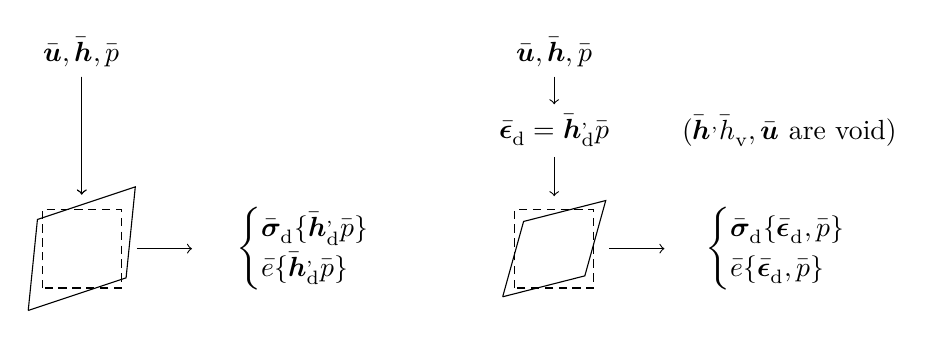
\begin{tikzpicture}[]
 \node (D) at (0,2.5) {$\bar{\ta u}, \bar{\ts h}, \bar p$};
 \draw[densely dashed] (-0.5,-0.5) rectangle (0.5,0.5);
 \draw[] (-0.679901, -0.785203) -- (0.562857, -0.370962) -- (0.679901, 0.785203) -- (-0.562857, 0.370962) -- (-0.679901, -0.785203);
 \node at (3,0) {$\begin{cases} \bar{\ts\sigma}_\dev\{\bar{\ts h}_\dev^\sym, \bar{p}\} \\ \bar{e}\{\bar{\ts h}_\dev^\sym, \bar{p}\}\end{cases}$};
 \draw[->] (D.south) -- +(0,-1.5);
 \draw[->] (D.south) -- +(0,-1.5);
 \draw[->] (0.7,0) -- (1.4,0);

 \begin{scope}[shift={(6,0)}]
 \draw[densely dashed] (-0.5,-0.5) rectangle (0.5,0.5);
 \draw[] (-0.654469, -0.611173) -- (0.388827, -0.345531) -- (0.654469, 0.611173) -- (-0.388827, 0.345531) -- (-0.654469, -0.611173);
 \node (A) at (0,2.5) {$\bar{\ta u}, \bar{\ts h}, \bar p$};
 \node (B) at (0,1.5) {$\bar{\ts \epsilon}_\dev = \bar{\ts h}_\dev^\sym, \bar{p}$};
 \node[anchor=west] at (1.5,1.5) {($\bar{\ts h}^\skw, \bar{h}_\vol, \bar{\ta u}$ are void)};
 \node at (3,0) {$\begin{cases} \bar{\ts\sigma}_\dev\{\bar{\ts\epsilon}_\dev, \bar{p}\} \\ \bar{e}\{\bar{\ts\epsilon}_\dev, \bar{p}\}\end{cases}$};
 \draw[->] (A.south) -- (B.north);
 \draw[->] (B.south) -- +(0,-0.5);
 \draw[->] (0.7,0) -- (1.4,0);
 \end{scope}
 
\end{tikzpicture}
 \caption{Comparison of the RVE-problem formulations; Original (left) and Canonical (right).}\label{fig:format_comparison}
\end{figure}
An illustrative comparison between the two RVE formulations are shown \Cref{fig:format_comparison}.
Despite the different displacement fields, the homogenized responses, $\bar{\ts\sigma}_\dev$ and $\bar{e}$, are the same.


%----------------------------------------------------------------------------
It follows from \cref{eq51} that the new variable $\bar{e}$ correctly obtains the value $\bar{e} = \homgen{\hat{e}(p)}$ in accordance with \cref{eq33b}.
%----------------------------------------------------------------------------------------------------------
Using these identities together with \cref{eq51b} and \cref{eq129a} we deduce
%--------------------------------------------------------------------------------------------------------
\begin{multline}
  \frac{|\Omega_\rve|}{|\Omega_\rve^\particle|}\homgen{ \hat{e}(p) - \ta u^\fluct\cdot\diff} 
          = \frac{|\Omega_\rve|}{|\Omega_\rve^\particle|}[c_\rve^*(p; 1)-\homgen{\ta u^\fluct\cdot\diff}]
          = \frac{|\Omega_\rve|}{|\Omega_\rve^\particle|}[-b_\rve(1, \ta u)-\homgen{\ta u^\fluct\cdot\diff}]
\\
          = \frac{|\Omega_\rve|}{|\Omega_\rve^\particle|}\homgen{[\ta u - \ta u^\fluct]\cdot\diff}
          = \bar{\ts\epsilon}_\dev\dprod\ts I + \bar{e}
          = \bar{e}
\end{multline}


\section{Variational properties of the RVE-problem -- Energy bounds from RVE-functional}

\subsection{Variational properties for the canonical formulation of the RVE-problem -- The RVE-potential}

In order to establish bounds on the homogenized properties based on the results from the Dirichlet and Neumann problems, we shall introduce an appropriate ``RVE-potential'' as follows:
%----------------------------------------------------------------------------------------------------------------
\begin{equation}
    \Pi_\rve(\bar{\ts\epsilon}_\dev,\bar{p};\ta{u},p,\ta{t},\bar{e}) =
    \Lambda_\rve(\ta{u},p) + \bar{p}\,\bar{e} +
    d_\rve(\ta{t},\ta{u}-\bar{\ts\epsilon}_\dev\cdot[\ta{x}-\bar{\ta{x}}]-\bar{e}\,\ta{x}_\mean)
\label{eq81}
\end{equation}
%----------------------------------------------------------------------------------------------------------------------
where $\Lambda_\rve(\ta{u},p)$ is the ``intrinsic'' energy potential that was defined in \cref{eqRveBulkPotential}.

We now define the volume-specific ``macroscale energy density''\footnote{$\bar{\psi}_\rve \to \bar{\psi}$, the ``effective energy density'', for sufficiently large RVE. } as the value of $\Pi_\rve$ at the following generalized saddle-point:
%----------------------------------------------------------------------------------------------------------------
\begin{equation}
    \bar{\psi}_\rve\epspargs =
    \inf_{\hat{\ta{u}}\in\set{U}_\rve}
    \sup_{\substack{ \hat{p}\in\set{P}_\rve \\ \hat{\ta{t}}\in\set{T}_\rve }}
    \inf_{ \hat{\bar{e}}\in\set{R} }
    \Pi_\rve(\bar{\ts\epsilon}_\dev,\bar{p};\hat{\ta{u}},\hat{p},\hat{\ta{t}},\hat{\bar{e}})
\label{eq:periodic_energy}
\end{equation}
%----------------------------------------------------------------------------------------------------------------------
A stationary point of $\Pi_\rve$ is defined by the relations
%----------------------------------------------------------------------------
\begin{subequations}\label{eq:rveStat}
\begin{alignat}{4}
    &(\Pi_\rve)'_u(\bar{\ts\epsilon}_\dev,\bar{p};\ta{u},p,\ta{t},\bar{e};\delta\ta{u}) &&= 0
    & \quad & \forall \delta\ta{u} &&\in\set{U}_\rve
\label{eq:rveStata} \\
    &(\Pi_\rve)'_p(\bar{\ts\epsilon}_\dev,\bar{p};\ta{u},p,\ta{t},\bar{e};\delta p) &&= 0
    & \quad & \forall \delta p &&\in\set{P}_\rve
\label{eq:rveStatb} \\
    &(\Pi_\rve)'_t(\bar{\ts\epsilon}_\dev,\bar{p};\ta{u},p,\ta{t},\bar{e};\delta\ta{t}) &&= 0
    & \quad & \forall \delta\ta{t} &&\in\set{T}_\rve
\label{eq:rveStatc} \\
    &(\Pi_\rve)'_{\bar{e}}(\bar{\ts\epsilon}_\dev,\bar{p};\ta{u},p,\ta{t},\bar{e};\delta \bar{e}) &&= 0
    & \quad & \forall \delta \bar{e} &&\in\set{R}
\label{eq:rveStatd}
\end{alignat}
\end{subequations}
%----------------------------------------------------------------------------
It is readily seen that the system in \cref{eq:rveStat} is precisely that of \cref{eq51}, and we may parameterize its solution as
%----------------------------------------------------------------------------------------------------------------
\begin{equation}
    \ta{u}=\ta{u}\epspargs, \,\,
    p=p\epspargs, \,\,
    \ta{t}=\ta{t}\epspargs, \,\,
    \bar{e}=\bar{e}\epspargs
\label{eq85}
\end{equation}
%----------------------------------------------------------------------------------------------------------------------
At the stationary point, we may use the result in \cref{eq:rveStatc} to conclude that
%----------------------------------------------------------------------------------------------------------------
\begin{equation}
    d_\rve(\ta{t}\epspargs,\ta{u}\epspargs-\bar{\ts\epsilon}_\dev\cdot[\ta{x}-\bar{\ta{x}}]-\bar{e}\epspargs\,\ta{x}_\mean) = 0
\label{eq86}
\end{equation}
%----------------------------------------------------------------------------------------------------------------------
whereby the energy at the stationary point is deduced to become
%----------------------------------------------------------------------------------------------------------------
\begin{equation}
    \bar{\psi}_\rve\epspargs =
    \Lambda_\rve(\ta{u}\epspargs,p\epspargs) + \bar{p}\,\bar{e}\epspargs
\label{eq87}
\end{equation}
%----------------------------------------------------------------------------------------------------------------------
We now deduce that $\bar{\psi}_\rve$ serves as the ``macroscale energy density'' for $\bar{\ts\sigma}_\dev$ and $\bar{e}$ in the sense that we have the macroscale constitutive relations
%----------------------------------------------------------------------------------------------------------------
\begin{equation}
    \bar{\ts\sigma}_\dev\epspargs = \frac{\partial \bar{\psi}_\rve\epspargs}{\partial \bar{\ts\epsilon}_\dev}, \quad
     \bar{e}\epspargs = \frac{\partial \bar{\psi}_\rve\epspargs}{\partial \bar{p}}
\label{eq88}
\end{equation}
%----------------------------------------------------------------------------------------------------------------------
Details of the proof are given in \Cref{appendix:macroEnergy}.

From the solution of the RVE-problem, $\bar{e}$ is obtained directly as a primary variable.
The deviatoric stress $\bar{\ts\sigma}_\dev$ is obtained by post-processing:
\begin{align}
 \bar{\ts\sigma}_\dev = \frac{1}{\volume} \int_{\Gamma_\rve^+} \ta t \outerp \jmp{\ta x - \bar{\ta x}}\dif S + \bar{p}\ts I
\label{eq:weak_periodic_sigma_dev}
\end{align}


\subsection{Variational properties for Dirichlet boundary conditions}

In order to establish a suitable variational setting we replace the solution space $\set{U}_\rve$ with $\set{U}_\rve^\Dirichlet\subseteq\set{U}_\rve$ defined as
%----------------------------------------------------------------------------
\begin{align}
    \set{U}_\rve^\Dirichlet &= \{\ta{v} \,|\,\, \ta{v}=\check{\ts\epsilon}_\dev\cdot[\ta{x}-\bar{\ta{x}}]+\check{e}\,\ta{x}_\mean+\ta{v}^\fluct, (\check{\ts\epsilon}_\dev,\check{e}, \ta v^\fluct)\in\set{R}^{3\times3}_\dev \times\set{R}\times\set{U}_\rve^{\Dirichlet,\fluct} \}
\label{eq61a} \\
\intertext{where}
    \set{U}_\rve^{\Dirichlet,\fluct} &= \{\ta{v}\in \set{U}_\rve^\fluct \,|\,\, \ta{v}=\ta{0} \text{ on } \Gamma_\rve \}
\label{eq61b}
\end{align}
%----------------------------------------------------------------------------
while $\set{P}_\rve^\Dirichlet=\set{P}_\rve$, ${\set{T}}_\rve^\Dirichlet={\set{T}}_\rve$ are the same spaces as for the generic problem.
The generalized saddle-point problem \cref{eq:periodic_energy} can now be rephrased as
%----------------------------------------------------------------------------------------------------------------
\begin{equation}
    \bar{\psi}_\rve^\Dirichlet\epspargs =
    \inf_{\substack{
    \hat{\ta{u}}^\fluct\in\set{U}_\rve^{\Dirichlet,\fluct}\\
    \check{\ts\epsilon}_\dev\in \set{R}^{3\times 3}_\dev \\
    \check{e}\in\set{R}
    }}
    \sup_{\substack{
    \hat{p}\in\set{P}_\rve\\
    \hat{\ta{t}}\in\set{T}_\rve
    }}
    \inf_{
    \hat{\bar{e}}\in\set{R}
    }
    \Pi_\rve(\bar{\ts\epsilon}_\dev,\bar{p};\check{\ts\epsilon}_\dev\cdot[\ta{x}-\bar{\ta{x}}] + \check{e}\,\ta{x}_\mean+\hat{\ta{u}}^\fluct,\hat{p},\hat{\ta{t}},\hat{\bar{e}})
\label{eq:dirichlet_energy}
\end{equation}
%----------------------------------------------------------------------------------------------------------------------
where
%----------------------------------------------------------------------------------------------------------------
\begin{multline}
    \Pi_\rve(\bar{\ts\epsilon}_\dev,\bar{p};\check{\ts\epsilon}_\dev\cdot[\ta{x}-\bar{\ta{x}}] + \check{e}\,\ta{x}_\mean+\hat{\ta{u}}^\fluct,\hat{p},\hat{\ta{t}},\hat{\bar{e}}) =
\\
    \Lambda_\rve(\check{\ts\epsilon}_\dev\cdot[\ta{x}-\bar{\ta{x}}] + \check{e}\,\ta{x}_\mean+\hat{\ta{u}}^\fluct,\hat{p}) + \bar{p}\,\hat{\bar{e}}
     + d_\rve(\hat{\ta{t}}, [\check{\ts\epsilon}_\dev-\bar{\ts\epsilon}_\dev]\cdot[\ta{x}-\bar{\ta{x}}]+[\check{e}-\hat{\bar{e}}]\,\ta{x}_\mean)
\label{eq91b}
\end{multline}
%----------------------------------------------------------------------------------------------------------------------
The only possibility to obtain a finite value of $\bar{\psi}_\rve^\Dirichlet$ while evaluating the sup over $\hat{\ta{t}}\in\set{T}_\rve$ is to set $\check{\ts\epsilon}_\dev = \bar{\ts\epsilon}_\dev$ and $\check{e} = \hat{\bar{e}}$.
Hence, we replace the saddle-point problem by
%----------------------------------------------------------------------------------------------------------------
\begin{equation}
    \bar{\psi}_\rve^\Dirichlet\epspargs =
    \inf_{
    \hat{\ta{u}}^\fluct\in\set{U}_\rve^{\Dirichlet,\fluct}
    }
    \sup_{
    \hat{p}\in\set{P}_\rve
    }
    \inf_{
    \hat{\bar{e}}\in\set{R}
    }
    \Pi_\rve^\Dirichlet(\bar{\ts\epsilon}_\dev,\bar{p};\hat{\ta{u}}^\fluct,\hat{p},\hat{\bar{e}})
\label{eq93a}
\end{equation}
%----------------------------------------------------------------------------------------------------------------------
where
%----------------------------------------------------------------------------------------------------------------
\begin{equation}
    \Pi_\rve^\Dirichlet(\bar{\ts\epsilon}_\dev,\bar{p};\hat{\ta{u}}^\fluct,\hat{p},\hat{\bar{e}})
    = \Lambda_\rve(\bar{\ts\epsilon}_\dev\cdot[\ta{x}-\bar{\ta{x}}]+\hat{\bar{e}}\,\ta{x}_\mean+\hat{\ta{u}}^\fluct,\hat{p}) - \bar{p}\,\hat{\bar{e}}
\label{eq93b}
\end{equation}
%----------------------------------------------------------------------------------------------------------------------
A stationary point of $\Pi_\rve^\Dirichlet$ is defined by the relations
%----------------------------------------------------------------------------
\begin{subequations}\label{eq94}
\begin{alignat}{4}
    &(\Pi_\rve^\Dirichlet)'_u(\bar{\ts\epsilon}_\dev,\bar{p};\ta{u}^\fluct,p,\bar{e};\delta\ta{u}^\fluct) &&= 0
    &\quad & \forall \delta\ta{u}^\fluct &&\in\set{U}_\rve^{\Dirichlet,\fluct}
\label{eq94a} \\
    &(\Pi_\rve^\Dirichlet)'_p(\bar{\ts\epsilon}_\dev,\bar{p};\ta{u}^\fluct,p,\bar{e};\delta p) &&= 0
    &\quad & \forall \delta p &&\in\set{P}_\rve
\label{eq94b} \\
    &(\Pi_\rve^\Dirichlet)'_{\bar{e}}(\bar{\ts\epsilon}_\dev,\bar{p};\ta{u}^\fluct,p,\ta{t},\bar{e};\delta\bar{e}) &&= 0
    &\quad & \forall \delta\bar{e} &&\in\set{R}
\label{eq94c}
\end{alignat}
\end{subequations}
%----------------------------------------------------------------------------
and this system of equations takes the explicit form: For given values $\bar{\ts\epsilon}_\dev, \bar{p}$, find the subscale fields $(\ta{u}^\fluct,p,\bar{e})\in\set{U}_\rve^{\Dirichlet,\fluct}\times\set{P}_\rve\times\set{R}$ that solve the system
%----------------------------------------------------------------------------
\begin{subequations}\label{eq:weak_form_dirichlet}
\begin{alignat}{3}
    a_\rve(\bar{\ts\epsilon}_\dev\cdot[\ta{x}-\bar{\ta{x}}]+\ta{u}^\fluct;\delta\ta{u}^\fluct) + b_\rve(p,\delta\ta{u}^\fluct) &= l_{\surf\rve}(\delta\ta{u}^\fluct)
    &\quad& \forall \delta\ta{u}^\fluct &&\in \set{U}_\rve^{\Dirichlet,\fluct}
\label{eq64a} \\
    b_\rve(\delta p,\ta{u}^\fluct) + b_\rve(\delta p,\bar{e}\,\ta{x}_\mean) + c^*_\rve(p;\delta p) &= 0
    &\quad& \forall \delta p &&\in \set{P}_\rve
\label{eq64b} \\
    b_\rve(p,\delta\bar{e}\,\ta{x}_\mean) &=
    - \bar{p}\,\delta\bar{e}
    &\quad& \forall \delta\bar{e} &&\in \set{R}
\label{eq64c}
\end{alignat}
\end{subequations}
%----------------------------------------------------------------------------
Finally, the macroscale energy density at the stationary point becomes
%----------------------------------------------------------------------------------------------------------------
\begin{equation}
    \bar{\psi}_\rve^\Dirichlet\epspargs =
    \Lambda_\rve(\bar{\ts\epsilon}_\dev\cdot[\ta{x}-\bar{\ta{x}}]+\bar{e}\epspargs\,\ta{x}_\mean+\ta{u}^\fluct\epspargs,p\epspargs) +\bar{p}\,\bar{e}\epspargs
\label{eq95}
\end{equation}
%----------------------------------------------------------------------------------------------------------------------

From the RVE-problem in \cref{eq:weak_form_dirichlet}, $\bar{e}$ is obtained directly as a primary variable.
The deviatoric stress $\bar{\ts\sigma}_\dev$ is obtained by post-processing:
\begin{align}
 \bar{\ts\sigma}_\dev = \frac{1}{\volume} \int_{\Gamma_\rve^+} \ta t \outerp \jmp{\ta x - \bar{\ta x}}\dif S + \bar{p}\ts I
\label{eq:weak_dirichlet_sigma_dev}
\end{align}
However in practice $\bar{\ts\sigma}_\dev$ is conveniently obtained as the reaction forces associated with the prescribed $\bar{\ts\epsilon}_\dev$.

\textbf{Remark}:
The VMCM in \cref{eq:macro_homogeneity_original} is still valid for the restricted space $\set{U}_\rve^{\Dirichlet,\fluct}\subset \set{U}_\rve^\fluct$.
Since $d_\rve(\delta\ta t^\fluct, \ta u^\fluct) = 0\;\forall\,\ta u^\fluct \in \set U_\rve^{\Dirichlet,\fluct}$, \cref{eq:macro_homogeneity_original_a} is satisfied for all $\delta\ta u^\fluct\in\set U^{\Dirichlet,\fluct}$. $\Box$

\subsection{Variational properties for Neumann boundary conditions}
The Neumann condition represents the weakest possible way of enforcing the micro-periodicity condition.
Here it is considered as a \emph{model assumption}; however, it is also possible to view this choice as a (crude) FE-approximation of the deviatoric traction field.
The pertinent RVE-problem is obtained from the general format upon restricting the space $\set{T}_\rve$, i.e.\ introducing $\set{T}_\rve^\Neumann\subseteq\set{T}_\rve$ defined as
%----------------------------------------------------------------------------
\begin{equation}
    \set{T}_\rve^\Neumann =
    \{\ta{t}\in\set{T}_\rve\,|\,\, \exists(\check{\ts\sigma}_\dev,\check{p})\in\set{R}^{3\times3}_\dev \times\set{R} \text{ s.t. }
    \ta{t}=\left[\check{\ts\sigma}_\dev-\check{p}\ts{I}\right]\cdot\ta{n} \text{ on } \Gamma_\rve^+\}
    \label{eq65}
\end{equation}
%---------------------------------------------------------------------------
while $\set{U}_\rve^\Neumann=\set{U}_\rve$ and $\set{P}_\rve^\Neumann=\set{P}_\rve$ are left unrestricted.
Clearly, the choice of $\set{T}_\rve^\Neumann$ restricts the tractions to become piecewise constant on each of the three positive boundary faces of the RVE-cube.
The generalized saddle-point problem \cref{eq:periodic_energy} can then be rephrased as
%----------------------------------------------------------------------------------------------------------------
\begin{equation}
    \bar{\psi}_\rve^\Neumann\epspargs =
    \inf_{
    \hat{\ta{u}}\in\set{U}_\rve
    }
    \sup_{\substack{
    \hat{p}\in\set{P}_\rve \\
    \check{\ts\sigma}_\dev\in\set{R}^{3\times3}_\dev \\
    \check{p}\in\set{R}
    }}
    \inf_{
    \hat{\bar{e}}\in\set{R}
    }
    \Pi_\rve(\bar{\ts\epsilon}_\dev,\bar{p};\hat{\ta{u}},\hat{p},\left[\check{\ts\sigma}_\dev-\check{p}\ts{I}\right]\cdot\ta{n},\hat{\bar{e}})
\label{eq:neumann_energy}
\end{equation}
%----------------------------------------------------------------------------------------------------------------------
where
%----------------------------------------------------------------------------------------------------------------
\begin{multline}
    \Pi_\rve(\bar{\ts\epsilon}_\dev,\bar{p};\hat{\ta{u}},\hat{p},\left[\check{\ts\sigma}_\dev-\check{p}\ts{I}\right]\cdot\ta{n},\hat{\bar{e}})
    =
\\
    \Lambda_\rve(\hat{\ta{u}},\hat{p}) + \bar{p}\,\hat{\bar{e}} +
    d_\rve(\left[\check{\ts\sigma}_\dev-\check{p}\ts{I}\right]\cdot\ta{n},\hat{\ta{u}}-\bar{\ts\epsilon}_\dev\cdot
    [\ta{x}-\bar{\ta{x}}]-\hat{\bar{e}}\,\ta{x}_\mean)
\label{eq96b}
\end{multline}
%----------------------------------------------------------------------------------------------------------------------
The only possibility to obtain a finite value of $\bar{\psi}_\rve^\Neumann$ while evaluating the $\inf$ over $\hat{\bar{e}}\in\set{R}$ is to set $\check{p} = \bar{p}$.
As a direct consequence the variable $\hat{\bar{e}}$ disappears in the resulting expression, cf.\ \cref{eq98b} below.
Moreover, from \cref{eq:weak_periodic_sigma_dev} we see that for tractions $\ta t \in \set T_\rve^\Neumann$ we obtain $\check{\ts\sigma}_\dev
= \homgen{ \hat{\ts{\sigma}}_\dev(\ts{\epsilon}_\dev[\ta{u}\epspargs]) } = \bar{\ts\sigma}_\dev\epspargs$.
%----------------------------------------------------------------------------------------------------------------------
Hence, we replace the saddle-point problem by
%----------------------------------------------------------------------------------------------------------------
\begin{align}
    \bar{\psi}_\rve^\Neumann\epspargs =
    \inf_{
    \hat{\ta{u}}\in\set{U}_\rve
    }
    \sup_{\substack{
    \hat{p}\in\set{P}_\rve \\
    \bar{\ts\sigma}_\dev\in\set{R}^{3\times3}_\dev
    }}
    \Pi_\rve^\Neumann(\bar{\ts\epsilon}_\dev,\bar{p};\hat{\ta{u}},\hat{p},\bar{\ts\sigma}_\dev)
%\nonumber \\
%    &=& \inf_{\tilde{\ta{u}}^\fluct\in\set{U}^{\Dirichlet,\fluct}} \sup_{\tilde{p}\in\set{P} \tilde{\ta{t}}\in\set{T}} \inf_{\check{e}\in\set{R}}
%    \left[\Lambda_\rve(\tilde{\ta{u}},\tilde{p}) - \bar{p}\,\check{e}\right]
\label{eq98a}
\end{align}
%----------------------------------------------------------------------------------------------------------------------
where
%----------------------------------------------------------------------------------------------------------------
\begin{equation}
    \Pi_\rve^\Neumann(\bar{\ts\epsilon}_\dev,\bar{p};\hat{\ta{u}},\hat{p},\bar{\ts\sigma}_\dev)
    = \Lambda_\rve(\hat{\ta{u}},\hat{p}) +
    d_\rve([\bar{\ts\sigma}_\dev-\bar{p}\ts{I}]\cdot\ta n,\hat{\ta{u}}-\bar{\ts\epsilon}_\dev\cdot[\ta{x}-\bar{\ta{x}}])
\label{eq98b}
\end{equation}
%----------------------------------------------------------------------------------------------------------------------
A stationary point of $\Pi_\rve^\Neumann$ is defined by the relations
%----------------------------------------------------------------------------
\begin{subequations}\label{eq104}
\begin{alignat}{4}
    &(\Pi_\rve^\Neumann)'_u(\bar{\ts\epsilon}_\dev,\bar{p};\ta{u},p,\bar{\ts\sigma}_\dev;\delta\ta{u}) &&= 0
    &\quad & \forall \delta\ta{u} &&\in\set{U}_\rve
\label{eq104a} \\
    &(\Pi_\rve^\Neumann)'_p(\bar{\ts\epsilon}_\dev,\bar{p};\ta{u},p,\bar{\ts\sigma}_\dev;\delta p) &&= 0
    &\quad & \forall \delta p &&\in\set{P}_\rve
\label{eq104b} \\
    &(\Pi_\rve^\Neumann)'_{\bar{\sigma}}(\bar{\ts\epsilon}_\dev,\bar{p};\ta{u},p,\bar{\ts\sigma}_\dev;\delta\bar{\ts\sigma}_\dev) &&= 0
    &\quad & \forall \delta\bar{\ts\sigma}_\dev &&\in\set{R}^{3\times3}_\dev
\label{eq104c}
\end{alignat}
\end{subequations}
%----------------------------------------------------------------------------
and this system of equations takes the explicit form: For given values $\bar{\ts\epsilon}_\dev, \bar{p}$, find the subscale fields $\ta{u},p,\bar{\ts\sigma}_\dev\in\set{U}_\rve\times\set{P}_\rve\times\set{R}^{3\times 3}_\dev$ that solve the system
%----------------------------------------------------------------------------
\begin{subequations}\label{eq67}
\begin{alignat}{3}
    a_\rve(\ta{u};\delta\ta{u}) + b_\rve(p,\delta\ta{u}) +  d_\rve(\bar{\ts\sigma}_\dev\cdot\ta n,\delta\ta{u}) &= d_\rve(\bar{p}\,\ta n,\delta\ta u) + l_{\surf\rve}(\delta\ta{u})
    & \quad & \forall \delta\ta{u} &&\in \set{U}_\rve
\label{eq67a} \\
    b_\rve(\delta p,\ta{u}) + c^*_\rve(p;\delta p) &= 0
    & \quad & \forall \delta p &&\in \set{P}_\rve
\label{eq67b} \\
    d_\rve(\delta\bar{\ts\sigma}_\dev\cdot\ta n,\ta{u}) &= - \bar{\ts\epsilon}_\dev\dprod\delta\bar{\ts\sigma}_\dev
    & \quad & \forall \delta\bar{\ts\sigma}_\dev &&\in\set{R}^{3\times3}_\dev
\label{eq67c}
\end{alignat}
\end{subequations}
%----------------------------------------------------------------------------
Finally, we obtain the macroscale energy density as
%----------------------------------------------------------------------------------------------------------------
\begin{equation}
    \bar{\psi}_\rve^\Neumann\epspargs =
    \Lambda_\rve(\ta{u}\epspargs,p\epspargs) + \bar{p}\,\homgen{ \ta{u}\epspargs\cdot\diff }
\label{eq105}
\end{equation}
%----------------------------------------------------------------------------------------------------------------------

From the RVE-problem in \cref{eq67}, $\bar{\ts\sigma}_\dev$ is obtained directly as a primary variable.
The volumetric strain $\bar{e}$ is obtained by post-processing:
\begin{align}
 \bar{e} = \frac{1}{\volume} \int_{\Gamma_\rve} \ta u \cdot \ta n\dif S.
\end{align}

\textbf{Remark}:
The VMCM in \cref{eq:macro_homogeneity_original} is still valid for the restricted space $\set{T}_\rve^\fluct = \{\ta 0\}$.
Since $d_\rve(\ta 0, \bullet) = 0$, \cref{eq:macro_homogeneity_original_a} is valid for all $\delta\ta u^\fluct \in \set U_\rve^\fluct$. $\Box$


\subsection{Macroscale tangent relations}
In order to solve the (generally nonlinear) macroscale problem \cref{eq:macro} in the FE\textsuperscript{2}-setting using Newton iterations, we need the pertinent tangent operators.
Linearizing the implicit relations $\bar{\ts\sigma}_\dev\epspargs$ and $\bar{e}\epspargs$ we obtain
\begin{align}
 \dif\bar{\ts\sigma}_\dev = \bar{\tf E} \dprod \dif\bar{\ts\epsilon}_\dev + \bar{\ts E}\, \dif\bar{p},
\quad
 \dif\bar{e} = \bar{\ts C} \dprod \dif\bar{\ts\epsilon}_\dev - \bar{C}\, \dif\bar{p}
\label{eq:periodic_difsigma}
\end{align}
thereby defining the tangents $\bar{\tf E}$ (4th order), $\bar{\ts E}$ (2nd order), $\bar{\ts C}$ (2nd order), and $\bar{C}$ (scalar).
Since a potential exists, it follows that $\bar{\tf {E}}$ possesses major symmetry and that $\bar{\ts E} = \bar{\ts C}$, cf.\ \"Ohman et. al \cite{ohman_computational_2012}.

In order to compute the tangent operators, it is necessary to first compute the relevant sensitivity fields w.r.t.\ changes of the macroscale variables $\bar{\ts\epsilon}_\dev$ and $\bar{p}$, and they are solved from the pertinent tangent problem.
On should then note that the particular sensitivity fields that are actually exploited (and needed) and the corresponding explicit formulation of the tangent problem depend on the chosen formulation of the RVE-problem (in terms of the boundary conditions: Weakly Periodic, Dirichlet, Neumann). 
Here, we shall give details only on the ``generic'' choice of the weakly periodic conditions.

\textbf{Remark}: In the case of macroscale incompressibility, $\bar{\ts C}$ and $\bar{C}$ will vanish. $\Box$

As a point of departure for computing the tangent tensors, we note that $\bar{e}\epspargs$ is a primary variable in the RVE-problem, whereas $\bar{\ts\sigma}_\dev\epspargs$ is post-processed via \cref{eq:weak_periodic_sigma_dev}.
We thus need to compute sensitivities of $\bar{e}$ and $\ta t$ from the tangent problem.
To begin with, we establish the linearized form of \cref{eq51} at the solution state to obtain
\begin{subequations}
\begin{alignat}{3}
    (a_\rve)'(\ta{u};\delta\ta{u},\dif\ta u) + b_\rve(\dif p,\delta\ta{u}) + d_\rve(\dif\ta{t},\delta\ta{u}) &= 0
    &\quad& \forall \delta\ta{u} &&\in \set{U}_\rve
\\
    b_\rve(\delta p,\dif\ta{u}) + (c^*_\rve)'(p;\delta p, \dif p) &= 0
    &\quad& \forall \delta p &&\in \set{P}_\rve
\\
    d_\rve(\delta\ta{t},\dif\ta{u}) - d_\rve(\delta\ta{t},\dif\bar{e}\,\ta{x}_\mean) &= d_\rve(\delta\ta{t},\dif\bar{\ts\epsilon}_\dev \cdot[\ta{x}-\bar{\ta{x}}])
    &\quad& \forall \delta\ta{t} &&\in \set{T}_\rve
\\
    - d_\rve(\dif\ta{t},\delta\bar{e}\,\ta{x}_\mean) &=
    - \dif\bar{p}\,\delta\bar{e}
    &\quad& \forall \delta\bar{e} &&\in \set{R}
\end{alignat}
\end{subequations}
which must be valid for any given perturbations $\dif\bar{\ts\epsilon}_\dev$ and $\dif\bar{p}$ giving rize to the corresponding perturbations $\dif\ta u$, $\dif p$, $\dif\ta t$, and $\dif\bar{e}$ in the solution fields.

Next, we introduce orthonormal base dyads $\ts G_i$, $i = 1,2,...,8$ to ensure that the deviatoric tensors $\ts\epsilon_\dev$ and $\ts\sigma_\dev$ are, indeed, deviatoric in character.
In other words we do not use the conventional base dyads $\ta e_i\outerp\ta e_j$, $i,j=1,2,3$, but we rather introduce the new set of base dyads such that the requirement $\ts G_i \dprod \ta I = 0$ for $i=1,2,...,8$ is fulfilled.
Examples of such (generally unsymmetric) dyads with Cartesian components, are
\begin{equation}
\begin{gathered}
 \ts G_1 = \frac{1}{\sqrt{6}}\left[\begin{smallmatrix} 2 & 0 & 0\\ 0 & -1 & 0\\ 0 & 0 & -1\end{smallmatrix}\right],\;
 \ts G_2 = \left[\begin{smallmatrix} 0 & 0 & 0\\ 0 & 1 & 0 \\ 0 & 0 & -1\end{smallmatrix}\right],\;
 \ts G_3 = \left[\begin{smallmatrix} 0 & 1 & 0\\ 0 & 0 & 0 \\ 0 & 0 & 0\end{smallmatrix}\right],\;
 \ldots,\;
 \ts G_8 = \left[\begin{smallmatrix} 0 & 0 & 0\\ 0 & 0 & 0 \\ 0 & 1 & 0\end{smallmatrix}\right].
\end{gathered}
\end{equation}
with respect to this basis, we have the representation
\begin{gather}
 \ts\epsilon_\dev = \sum_k (\ts\epsilon_\dev)_k \, \ts G_k,\quad 
 (\ts\epsilon_\dev)_k = \ts G_k \dprod \ts\epsilon_\dev
\\
 \ts\sigma_\dev = \sum_k (\ts\sigma_\dev)_k \, \ts G_k,\quad
 (\ts\sigma_\dev)_k = \ts G_k \dprod \ts\sigma_\dev
\end{gather}
% Hence, the component form of \cref{eq:periodic_difsigma} becomes
% \begin{align}
%  (\dif\ts\sigma_\dev)_i = \sum_k (\bar{\tf E})_{ik} (\dif\bar{\ts\epsilon}_\dev)_k + (\bar{\ts E})_i\dif\bar{p}
% \end{align}
% and
% \todo{why for E but not C}
% \begin{align}
%  \bar{\tf E} = \sum_{i,j} (\bar{\tf E})_{ij} \ts G_i \outerp \ts G_j,\quad \bar{\ts E} = \sum_i (\bar{\ts E})_i \ts G_i
% \end{align}
Next, we express the pertinent sensitivities via the representations
\begin{subequations}
\begin{align}
 \dif\ta u &= \sum_k \ta u_\ded^{(k)} (\dif\bar{\ts\epsilon}_\dev)_k + \ta u_\dep\,\dif\bar{p}
\\
 \dif p &= \sum_k p_\ded^{(k)} (\dif\bar{\ts\epsilon}_\dev)_k + p_\dep\,\dif\bar{p}
\\
 \dif\ta t &= \sum_k \ta t_\ded^{(k)} (\dif\bar{\ts\epsilon}_\dev)_k + \ta t_\dep\,\dif\bar{p}
\label{eq:periodic_dif_t}
\\
 \dif\bar{e} &= \sum_k \bar{e}_\ded^{(k)} (\dif\bar{\ts\epsilon}_\dev)_k + \bar{e}_\dep\,\dif\bar{p}
\label{eq:periodic_dif_ebar}
\end{align}
\end{subequations}
We thus obtain the following sets of tangent problems:
\begin{itemize}
 \item $\dif\bar{\ts\epsilon}_\dev = \ts G_k$ while $\dif\bar{p} = 0$: For $k = 1, \ldots, 8$, solve for the sensitivities $\ta{u}_\ded^{(k)}$, $p_\ded^{(k)}$, $\ta{t}_{\ded}^{(k)}$, $\bar{e}_\ded^{(k)}$ from the system 
\end{itemize}
\begin{subequations}\label{eq:p_sensitivities_d}
\begin{alignat}{3}
    (a_\rve)'(\ta{u};\delta\ta{u},\ta{u}_\ded^{(k)}) + b_\rve(p_\ded^{(k)},\delta\ta{u}) + d_\rve(\ta{t}_{\ded}^{(k)},\delta\ta{u}) &= 0
    &\quad& \forall \delta\ta{u} &&\in \set{U}_\rve
\\
    b_\rve(\delta p,\ta{u}_\ded^{(k)}) + (c^*_\rve)'(p;\delta p, p_\ded^{(k)}) &= 0
    &\quad& \forall \delta p &&\in \set{P}_\rve
\\
    d_\rve(\delta\ta{t},\ta{u}_\ded^{(k)}) - d_\rve(\delta\ta{t},\bar{e}_\ded^{(k)}\,\ta{x}_\mean) &= d_\rve(\delta\ta{t}, \ts G_k \cdot[\ta{x}-\bar{\ta{x}}])
    &\quad& \forall \delta\ta{t} &&\in \set{T}_\rve
\\
    - d_\rve(\ta{t}_{\ded}^{(k)},\delta\bar{e}\,\ta{x}_\mean) &= 0
    &\quad& \forall \delta\bar{e} &&\in \set{R}
\end{alignat}
\end{subequations}
\begin{itemize}
\item $\dif\bar{p} = 1$ while $\dif\bar{\ts\epsilon}_\dev = \ts 0$: Solve for the sensitivities $\ta{u}_\dep$, $p_\dep$, $\ta{t}_\dep$, $\bar{e}_\dep$ from the system 
\end{itemize}
\begin{subequations}\label{eq:p_sensitivities_p}
\begin{alignat}{3}
    (a_\rve)'(\ta{u};\delta\ta{u},\ta{u}_\dep) + b_\rve(p_\dep,\delta\ta{u}) + d_\rve(\ta{t}_\dep,\delta\ta{u}) &= 0
    &\quad& \forall \delta\ta{u} &&\in \set{U}_\rve
\\
    b_\rve(\delta p,\ta{u}_\dep) + (c^*_\rve)'(p;\delta p, p_\dep) &= 0
    &\quad& \forall \delta p &&\in \set{P}_\rve
\\
    d_\rve(\delta\ta{t},\ta{u}_\dep) - d_\rve(\delta\ta{t},\bar{e}_\dep\,\ta{x}_\mean) &= 0
    &\quad& \forall \delta\ta{t} &&\in \set{T}_\rve
\\
    - d_\rve(\ta{t}_\dep,\delta\bar{e}\,\ta{x}_\mean) &=
    - \delta\bar{e}
    &\quad& \forall \delta\bar{e} &&\in \set{R}
\end{alignat}
\end{subequations}
Now, upon linearizing \cref{eq:weak_periodic_sigma_dev} and using the representation for $\dif\ta t$ in \cref{eq:periodic_dif_t}, we obtain
\begin{align}
    \dif\bar{\ts\sigma}_{\dev}
    & =
    \frac{1}{\volume} \int_{\Gamma_\Box^+} \dif\ts t \outerp \jmp{\ta x - \bar{\ta x}}\dif S + \dif\bar{p}\ts I
\\
    &= 
    \underbrace{\sum_k \frac{1}{\volume} \int_{\Gamma_\Box^+} \ts t_\ded^{(k)} \outerp \jmp{\ta x - \bar{\ta x}}\dif S\outerp \ts G_k}_{\bar{\tf E}}\dprod\dif\bar{\ts\epsilon}_\dev + 
    \underbrace{\left[\frac{1}{\volume} \int_{\Gamma_\Box^+} \ts t_\dep \outerp \jmp{\ta x - \bar{\ta x}}\dif S + \ts I \right]}_{\bar{\ts E}}\dif\bar{p}
\end{align}
Directly from \cref{eq:periodic_dif_ebar}, we obtain
\begin{align}
 \dif\bar{e} = \underbrace{\sum_k \bar{e}_\ded^{(k)}\, \ts G_k}_{\bar{\ts C}} \dprod \dif \bar{\ts\epsilon}_\dev + \underbrace{\bar{e}_\dep}_{-\bar{C}}\,\dif\bar{p}
\end{align}

Macroscale tangent relations for the Dirichlet and Neumann boundary conditions are detailed in \Cref{appendix:sensitivity}.

\subsection{Bounds on the macroscale energy density}

Since we have derived the Dirichlet and Neumann problems by respectively restricting the solution spaces as
\begin{align}
 \set{U}_\rve^\Dirichlet \subset \set{U}_\rve,\quad \set{T}_\rve^\Neumann \subset \set{T}_\rve
\end{align}
it follows from \cref{eq:dirichlet_energy}, \cref{eq:neumann_energy}, and \cref{eq:periodic_energy} that
\begin{align}
 \bar\psi^\Dirichlet_\rve\{\bar{\ts\epsilon}_\dev, \bar{p}\} \geq \bar\psi\{\bar{\ts\epsilon}_\dev, \bar {p}\} \geq \bar\psi^\Neumann\{\bar{\ts\epsilon}_\dev, \bar {p}\}.
\end{align}
In other words, the Dirichlet and Neumann boundary conditions represent upper and lower bounds
on the macroscale energy density that is obtained with periodic boundary conditions for any given realization of the RVE and for a given macroscale state $(\bar{\ts\epsilon}_\dev, \bar{p})$.

In the case of linear elasticity, the tangent operators represent the upscaled (=homogenized) constant operators in the representations
\begin{align}
 \bar{\ts\sigma}_\dev = \bar{\tf E} \dprod \bar{\ts\epsilon}_\dev + \bar{\ts E}\, \bar{p}, \quad \bar{e} = \bar{\ts C}\dprod\bar{\ts\epsilon}_\dev - \bar{C}\,\bar{p}
\end{align}
whereby we obtain
\begin{alignat}{4}
 &\bar{\psi}_\rve\{\bar{\ts\epsilon}_\dev, \bar{p}\} &&= \frac12 \bar{\ts\epsilon}_\dev \dprod \bar{\tf E}\dprod \bar{\ts\epsilon}_\dev -\frac12 \bar{p}\;\bar{C}\;\bar{p}
&\quad&\forall\;\bar{\ts\epsilon}_\dev,\,\bar{p} &&\implies
 \bar{\tf E}^\Dirichlet \geq \bar{\tf E} \geq \bar{\tf E}^\Neumann,\quad
 \bar{C}^\Dirichlet \leq \bar{C} \leq \bar{C}^\Neumann
\end{alignat}



\section{Numerical results}

\begin{figure}[H]
 \centering
 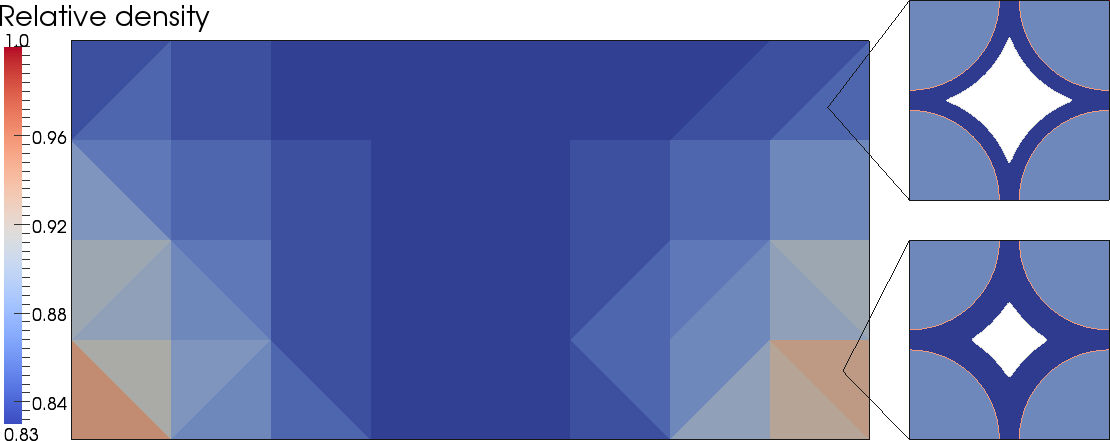
\includegraphics[width=\linewidth]{figures/macro_fe2_0000}
 \caption{FE2}
 \label{fig:final_dirichlet}
\end{figure}

\begin{figure}[H]
 \centering
 \begin{tikzpicture}
  \node at (0,0) {
\includegraphics[scale=0.15]{figures/initial_rve}};
  \node at (4,2) {
\includegraphics[scale=0.15]{figures/final_dirichlet}};
  \node at (4,-2) {
\includegraphics[scale=0.15]{figures/final_neumann}};
  \node at (0,1.5) {Initial};
  \node at (4,3.5) {Dirichlet};
  \node at (4,-0.5) {Neumann};
  \draw[-latex] (1.5,0.5) -- (2.5,1);
  \draw[-latex] (1.5,-0.5) -- (2.5,-1);
  \node at (8,2) {
\includegraphics[scale=0.2]{figures/rve_dirichlet_2}};
  \node at (8,-2) {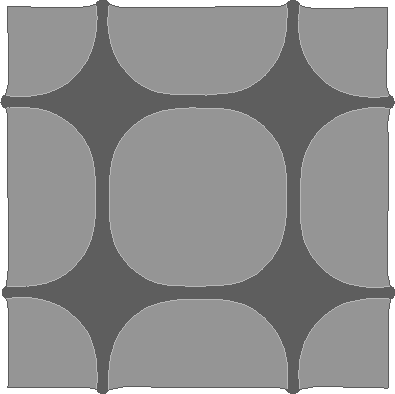
\includegraphics[scale=0.2]{figures/rve_neumann_2}};
 \end{tikzpicture}
 \caption{Initial and final state of RVEs subject to free sintering}
 \label{fig:final_neumann}
\end{figure}

\begin{figure}[H]
 \centering
\begin{tikzpicture}
 \begin{axis}[
    width=0.8\linewidth,
    height=0.4\linewidth,
    ylabel={Relative density [\%]},xlabel={Time (scaled)},
    xmax=1, xmin=0, ymax=1.01, ymin=0.83,
    cycle list name=linestyles,
    yticklabel style={font=\tiny}, xticklabel style={font=\tiny},
%     scaled y ticks=manual:{}{\pgfmathparse{#1*100}}, % Scale for percentage
%     scaled x ticks=manual:{}{\pgfmathparse{#1*1000}}, % Scale for percentage
    legend style={draw=black,rounded corners=3pt,font=\footnotesize},
    legend pos=south east
    ]
  \addplot[blue ,densely dashed] table[y index=2] {figures/macro_3_dirichlet_x.out.matdata};
  \addlegendentry {Dirichlet 3$\times$3}
  \addplot[red  ,densely dashed] table[y index=2] {figures/macro_2_dirichlet_x.out.matdata};
  \addlegendentry {Dirichlet 2$\times$2}
  \addplot[black,densely dashed] table[y index=2] {figures/macro_1_dirichlet_x.out.matdata};
  \addlegendentry {Dirichlet 1$\times$1}

  \addplot[blue ] table[y index=2] {figures/macro_3_neumann_x.out.matdata};
  \addlegendentry {Neumann 3$\times$3}
  \addplot[red  ] table[y index=2] {figures/macro_2_neumann_x.out.matdata};
  \addlegendentry {Neumann 2$\times$2}
  \addplot[black] table[y index=2] {figures/macro_1_neumann_x.out.matdata};
  \addlegendentry {Neumann 1$\times$1}
 \end{axis}
\end{tikzpicture}
 \caption{Evolution of porosity with time for a 1$\times$1 and 2$\times$2 unit-cell RVE subjected to zero macroscopic pressure, $\bar{p} = 0$.}
 \label{fig:porosity}
\end{figure}

\end{document}